\documentclass[letterpaper,12pt]{article}

% csm-thesis automatically includes the following packages:
%% float
%% setspace
%% geometry
%% graphics
%% textcase
%% subfig

% Note: Two package options exist for your convenience: ``insane'' and ``nolabel''.  To use these options together separate them by a comma, ie. \usepackage[insane,nolabel]{csm-thesis}
% * \usepackage[insane]{csm-thesis}
% Turn off all document sanity checks.  This option can be used to render a ``sub-document'' that is part of the root thesis document.  It is important to note that you should NEVER disable this check on your root thesis document, as important format errors and warnings will be disabled.
% * \usepackage[nolabel]{csm-thesis}
% Disables automatic reference ``labeling'' of figures and tables.  By default the thesis template prepends any reference to a figure or table with ``Figure~'' or ``Table~''.  This option is meant for disabling the labeling behavior when a document already has the appropriate labeling.  It is important to note that if your document DOES NOT have the appropriate labeling (the reference label must EXACTLY MATCH the caption label) then it will not pass the format review.
\usepackage{csm-thesis}

% For inserting large multi-page tables:
\usepackage{array}
\usepackage{longtable}
\usepackage{algpseudocode}
\usepackage{algorithm}
\usepackage{wrapfig}

% For inserting sideways tables and figures
\usepackage{rotating}
\usepackage[numbers]{natbib}
\graphicspath{{./images/}}
\usepackage{hyperref}

% For inserting programming code:
\usepackage{listings}

% For inserting landscape-mode objects:
\usepackage{pdflscape} % use ``lscape'' if you are not creating a PDF output

% For matrices:
\usepackage{amsmath}
\usepackage{caption}

\title{A method for improved ensemble forecasting for human traffic systems}

\degreetitle{Doctor of Philosophy}
\discipline{Computer Science}
\department{Electrical Engineering and Computer Science}

\author{James Howard}
\advisor{Dr. William Hoff}
\dpthead{Dr. Big Boss}{Professor and Head}

\begin{document}

% Parts of a Thesis
\frontmatter

\maketitle
\newpage

%%%% Parts of a Thesis - Front Matter - Copyright Page (optional)
%% If the copyright for your document spans multiple years, or does not match the current year, then replace ''\the\year`` below with the appropriate text.
\makecopyright{\the\year}
\newpage

%%% Parts of a Thesis - Front Matter - Signature Page (required)

\makesubmittal
\newpage

%%% Parts of a Thesis - Front Matter - Abstract (required)
\begin{abstract}
Forecasting the occupancy of buildings can lead to significant improvement of smart heating and cooling systems. Using a sensor network of simple passive infrared motion sensors densely placed throughout a building, we perform data mining to forecast occupancy a short time ($i.e.$, up to 60 minutes) into the future.  Our approach is to train a set of standard forecasting models to our time series data.  Each model then forecasts occupancy a various horizons into the future.  We combine these forecasts using a modified Bayesian combined forecasting approach.  The method is demonstrated on two large building occupancy datasets, and shows promising results for forecasting horizons of up to 60 minutes.  Because the two datasets have such different occupancy profiles, we compare our algorithms on each dataset to evaluate the performance of the forecasting algorithm for the different conditions.
\end{abstract}

\newpage

%%% Parts of a Thesis - Front Matter - Table of Contents (required)

\tableofcontents
\newpage

%%% Parts of a Thesis - Front Matter - List of Figures (if applicable)
%%% Parts of a Thesis - Front Matter - List of Tables (if applicable)

\listoffiguresandtables
\newpage

%\listofsymbols
%Place symbols here

\newpage

%%% Parts of a Thesis - Front Matter - List of Abbreviations (if applicable)
\listofabbreviations*
\newpage

\addabbreviation{Seasonal auto regressive moving average}{SARIMA}
\addabbreviation{Support vector machine}{SVM}
\addabbreviation{Time delayed neural network}{TDNN}
\addabbreviation{Bayesian combined forecaster}{BCF}
\addabbreviation{Anomaly bayesian combined forecaster}{ABCF}


%%% Parts of a Thesis - Front Matter - Acknowledgments (optional)
\begin{acknowledgments}
That you everyone
\end{acknowledgments}
\newpage

%%% Parts of a Thesis - Front Matter - Dedication (optional)

\begin{dedication}
For those that shall follow after.

TODO Fill in a dedication
\end{dedication}
\newpage

% Parts of a Thesis - Body

\bodymatter

%%% Parts of a Thesis - Body - All Chapters and Sections (required)
%Introduction
\chapter{Introduction}
According to the U.S. Department of Energy \cite{DOE2010}, energy for heating and cooling accounts for approximately 35 - 45\% of the total expenditure within a building.  With such a large investment of energy being used to regulate the temperature of a building, possible areas of improvement are heavily sought after.  Fully automated buildings with control systems to automatically heat and cool individual rooms or spaces have been designed \cite{Balan2009, Gwerder2008} to reduce building energy usage while maintaining proper temperatures throughout the building.  These systems are complex and require knowledge of room usage, and in more complex systems room occupancy, as inputs into system control models.
	
While many factors such as ambient temperature, ventilation air flow, room volume, \textit{etc.} affect the time it takes to heat or air condition a room, it still takes on the order of many minutes to bring a room to a stable desired temperature \cite{yang2004}.  Due to this lag in changing the temperature of a room, it is not sufficient for control systems to begin air conditioning a room upon initial occupancy.   Thus, to ensure that room temperatures are appropriate, smart building control systems typically rely on set schedules of occupancy.  These systems may use scheduled occupancy up to 24 hours into the future to determine current heating and air conditioning control \cite{Ma2010}.  

However, what happens to the system when building traffic deviates from its schedule?  Let us consider a university classroom building.  While not often, professors will occasionally cancel class.  What should a smart control system do during this time?  It does not make sense for the system to heat or cool the room as though it was occupied.  The system should adapt to the changing environment.  Similarly, what happens if snow has caused many of the students and faculty to stay at home?  In this case, a cancelled class in the morning is likely correlated to class cancellations later in the day.  Ideally the building control system should identify situations where there is a significant deviation in the number of occupants within any part of the building and modify its heating or cooling schedule to account for such situations.  In both of these scenarios, a set schedule is insufficient to produce an optimal heating or cooling schedule for the building.

As another example of the usage of complex control systems, consider the roadways of the United States.  Optimal timing of traffic lights on major roadways across the United States could result in approximately a 22\% reduction in emissions along with a 10\% reduction in fuel consumption \cite{DOT2007}.  As of 2005 the total estimated fuel savings would amount to approximately 17 billions gallons of motor fuels annually.  This traffic light timing does not only consider city lights, but also takes into account freeway onramp volume lights.

In the United States, traffic light timings are often determined by an individual from the local department of transportation standing near the light and manually determining a timing schedule, or in some cases multiple schedules to account for peak traffic times and non-peak times \cite{Koonce2008}.  These schedules are then fixed and are changed either when roadways change to make new timings necessary or if petitioned by local citizens.  These timings are then either set in local control box for that traffic light or by a central control system for the city.  

As with the building scenario, what happens when the traffic deviates from normal?  Fixed timings will not be able to account for changes in traffic.  Inclement weather scenarios should likely require different timings then sunny days.  Lights near large sporting events likely require different timings during those events than typical evenings.  Even if schedules were made for such scenarios, there certainly exist scenarios for which schedules can not be made manually such as lane blockages due to accidents. 

In both of the above environments, the control systems have to account for future occupancy of the environment.  It is inadequate for these systems to use only current data to control the system.  Accurate forecasts of the systems usage are necessary to produce optimal control systems.  

%Problem Statement
\subsection{Problem and objective}
As alluded to with the above examples, our focus is on improving forecasting accuracy on human controlled traffic systems.  By “traffic”, we mean the movement of vehicles along a road network, the movement of people in a building, or similar data derived from the actions of a group of people.  Overall, our method is more general than just traffic systems and we believe it will work with any dataset which has rare repeated events that lead to similar effects in the system.  For the rest of this paper, we define a time series dataset as $\{x_{t}^{(m)}\}$.  Each $x_{t}^{m}$ is an aggregate of the readings from sensor $m$ reading at time block $t$.  Our objective in this work is then:

\begin{enumerate}
	\item Produce an accurate forecast for $x_{t}^{(m)}$ $\delta$ time steps into the future.
	\item Reduce worst case forecasts.
	\item Keep approach unsupervised.
\end{enumerate}

Because the literature on forecasting is so vast, we specifically focus only on human traffic systems.  As we will demonstrate shortly, our approach will make some assumptions based on the type of data produced by these traffic systems which will   As a result, we will demonstrate considerably better results that would likely be possible with data from other sources.  Also, we will demonstrate our results empirically.  Due our lack of theoretical constraints, our improved results may simply be a by product of our datasets and and not something that may be applicable to other human traffic systems.  Of course, we do not believe this to be the case due to the improvement in vastly different datasets which we will demonstrate later.


%Give a sample example of the broncos game here and then discuss the need for worst case forecasts.
\subsubsection{A motivating example}

To illustrate an example of the need to minimize worst case forecasts, we present the following example.  The Denver Broncos, as with most American Football teams are a significant local attraction.  In 2010 the team had an average attendance of 74,908 \cite{ESPN2013}.  This attendance, combined with additional fans flooding downtown to patronize bars and restaurants creates an interesting effect on freeway traffic patterns.  Unsurprisingly, prior to the game there is an increase in total traffic volume along a freeway which is near the Broncos' Stadium.  Also, there exists a nearly 20\% drop in total traffic volume along the same stretch of freeway during the game.  ~\ref{fig:broncos} shows the total counts of Denver traffic by a single loop detector on a stretch of highway near the station for each hour of the day averaged for the first four Sunday Broncos home games and for the first four Sunday away games in 2010.  Comparing ~\ref{fig:broncos_off} with figure~\ref{fig:broncos_on} it is evident that a noticeable change in traffic patterns occur from approximately noon until approximately 6:00 pm.  This traffic change corresponds with a 2:05pm kickoff time for the game.

\begin{figure}[!ht]
	\begin{center}
		\subfigure[] {
			\includegraphics[width=0.49\textwidth]{broncos_off4.png}
			\label{fig:broncos_off}
		}
		\subfigure[] {
			\includegraphics[width=0.49\textwidth]{broncos4.png}
			\label{fig:broncos_on}
		}
	\end{center}
	\caption{Total number of cars passing major highway sensors in Denver on Sundays in September and October 2010}
	\label{fig:broncos}
\end{figure}

Such a significant difference in traffic patterns should lead to a change in traffic light control.  We have all likely encountered the frustrating scenario of attempting to leave one of these sporting events.  Traffic lights are often still on predefined timings and the situation arises where a large number of vehicles attempt to get through a traffic light controlled intersection in one direction with almost no vehicles attempting to get through the intersection in the perpendicular direction.  Ideally the light timings should be changed to fix this scenario and increase the green light time in the direction with multiple cars.  Of course, optimally other light timings will also need to be changed to account for the increase volume of traffic along certain paths within the city.

Traditional parametric forecasting models have difficulty accounting for these different traffic patterns and the problem becomes more difficult when when it is considered that the Broncos may play a Sunday night game or a Monday night game.  Thus our another goal of our approach is to handle these significant deviations from normal traffic patterns which are typically the causes of worse case forecasting scenarios.


\subsection{Approach}
To satisfy our first objective of producing an accurate forecast for dataset $x_{t}^{(m)}$ $\delta$ time steps into the future, we have created an ensemble forecasting model based on the Bayesian combined forecaster (BCF) created by Petridis \cite{Petridis2001}.  Chapter \ref{ch:BCF} discusses modifications we have made to BCF which improve its performance on human controlled traffic systems.  

To satisfy our second objective of reducing worst case forecasts, i.e. the sporting event scenario, we introduce a novel forecasting technique based on anomaly detection and modeling.  Empirically we have found that for human controlled traffic systems large deviations in forecasting accuracy often coincided with human controlled activities.  For the purposes of this paper, we frequently interchange the terms activities and anomalies.  The reason for this is as a matter of perspective.  To a forecasting model, an infrequently occurring human activity will likely produce anomalous results.  We describe any event which causes large prediction errors for our forecasting system as either an anomaly or an activity.  For vehicle traffic systems these activities might be sporting events, road closures, or accidents.  In the case of building models, such activities might be large infrequent meetings, cancelled classes, or early closure due to holidays.

Because such activities can overlap or occur at different times with varying amount of background noise present, it is a difficult task for one parametric model to accurately encapsulate all of the activities which occur within the system.  Our approach is to split the problem of forecasting into two parts: development of a background model and the development of a set of activity models.  Our background model is represented by any forecasting model.  In practice we have computed our results using traditional forecasting models such as Time Delayed Neural Networks, Auto Regressive Models or Support Vector Machines.   

To model activities, we propose comparing different models from the activity recognition literature along with a new model which we propose here.  Forecasting is then performed using an ensemble predictor defined in Chapter 5, taking outputs from all trained activity models and the background model.  ~\ref{fig:alg_overview} shows the general structure of our approach.  We combine classic forecasting models with activity models in a novel ensemble model to improve overall forecasting accuracy.

\begin{figure}
	\centering
	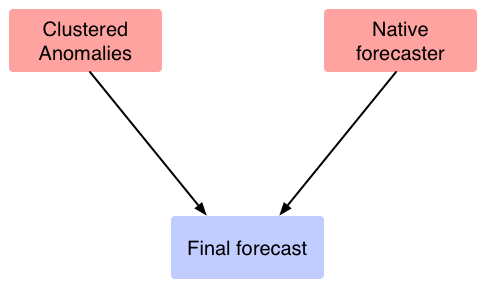
\includegraphics[width=0.5\textwidth]{simple_approach_overview.png}
	\caption{High level overview of our approach}
	\label{fig:alg_overview}
\end{figure}

Finally, in satisfying our third objective, we keep everything unsupervised.  Nothing in our approach prevents the use of supervised modeling of activities and incorporating a trained activity model into our final forecast, but such supervised information is not necessary to achieve improved forecasting results.


\subsection{Contributions}  
The contributions to the field of unsupervised traffic forecasting from this work are:
\begin{itemize}
\item{Extraction and modeling of forecasting activity models using residual errors from another forecasting model.}
\item{An improvement to a combined Bayesian prediction model to improve forecasting accuracy}
\item{A combined prediction model using an ensemble forecaster and activity models to improve short term forecasts during the presence of anomalous activities}
\end{itemize}

\subsection{Structure of the thesis}
The remainder of this thesis is outlined as follows: Chapter 2 defines typical forecasting models which are to be used for comparison and as base native forecasters for our final ensemble forecaster.  This chapter also introduces some notation used through this document.  Chapter 3 discusses the datasets used therein along with specifics details on any necessary changes to make the datasets compatible with our forecasters.  Chapter 4 discusses a classic ensemble forecaster which we apply to our datasets along with introducing some improvements on this forecaster which greatly improve its long term forecasting performance.  Finally Chapter 5 discusses our novel approach using activity modeling to improve the short term accuracy of any of our base forecaster for our datasets.  This section also includes a brief discussion of previous work in the realm of anomaly detection.

\chapter{Models}
With this chapter we explore some of the most common forecasting models for traffic datasets.  These models are meant to be used as a baseline from which to compare our results. Also in this chapter, we introduce the metrics which will be used for our analysis.  We feel this analysis useful to empirically demonstrate the various forecasting capabilities of these established models.

\subsection{Notation}
As already stated, we define a time series dataset used within as  $\{x_{t}^{(m)}\}$.  Each $x_{t}^{m}$ is an aggregate of the readings from sensor $m$ reading at time block $t$.  In total the number of time blocks are represented by $N$.

Forecasts for a given model $k$ from the set of all models $K$ are represented by 
\begin{equation}
y_{t + 1}^{k, m} = f(x_{t}, ..., x_{1}; \theta_{k}).
\end{equation}
\noindent
Thus the forecast of $x_{t + 1}$ is a function of all past data and some trained parameterization $\theta_{k}$ for that model.  For this work we forecast a model for each individual sensor and for convenience often drop the $m$ and $k$ from our forecast notation.  Also, in this work we need to forecast more than one time step into the future.  Future forecasts are performed through iterative one step ahead forecasts.    An example of a forecast two time steps ahead of current time $t$ is given by 
\begin{equation}
y_{t + 2} = f(y_{t + 1}, x_{t}, ..., x_{1}; \theta_{k}).
\end{equation}
\noindent
Such a forecast is simply the forecast for one time step into the future but now with the forecasted value of $y_{t + 1}$ used as the most recent datapoint to forecast $y_{t + 2}$.  Forecasting in this nature allows for forecasts any number of time steps into the future.

Another useful time series used in this work is the residual dataset defined as
\begin{equation}
r_{t,\delta} =  x_{t + \delta} - y_{t + \delta}.
\end{equation}
This set of residuals is the difference between the raw data and a forecasting function operating $\delta$ time steps into the future. 


\subsection{Forecast Error Measurements}
There are a multitude of various forecasting error measurements that have been used to assess forecast accuracy.  Expert recommendation of which forecast error measurement to use for what types of data has changed over time.  Armstrong \cite{Armstrong2001, Yokuma1995} found that root mean squared error (RMSE) was by far the most popular error measurement in 1981 among academics.  However, by 1995 RMSE preference by academics had dropped by roughly half and mean absolute percentage error (MAPE) was the preferred error measurement. 

For this work, to coincide with expert opinion on forecast error measurements, we use both mean absolute scale error (MASE) \cite{Hyndman2006, Hyndman2006a} and RMSE as cost functions to compare our forecasting accuracy.  RMSE was selected due to its simplicity and ubiquity within the forecasting community.  MASE was selected for it being both a modern derivation of MAPE and for its accuracy in places where MAPE does not provide adequate results.  

Also, because much of the focus of our work is interested in reducing inaccurate forecasts during the presence of some anomalous event, we introduce another forecasting measurement which we call root mean squared error outside of noise against naive (RMSEONAN).  This metric provides a convenient way to measure the improvement our approach yields which is not easily captured by RMSE and MASE.

\bigskip
\noindent \textbf{RMSE} \\
One of the most common error functions used to determine the quality of a set of forecasts.  It measures the average difference between two time series.  Due to its squared error term, this measurement is not a good indicator of error between distinctly different datasets.  For our work comparing the input series $x$ and the forecast series $y$ RMSE performs adequately.
\begin{equation}
RMSE_{\delta} = \sqrt{\frac{\sum_{t = 1}^{N - \delta}{(x_{t + \delta} - y_{t + \delta})^{2}}}{N - \delta}}
\end{equation}

\bigskip
\noindent \textbf{MASE} \\
Mean absolute scaled error was developed to be a generally applicable measurement of forecast error.  The metric is especially useful for datasets with intermittent demand unlike the commonly used MAPE score.  The reason it works well with intermittent time is that it will not return undefined or infinite values unless the compared datasets are equal \cite{Hyndman2008}.

\begin{equation}
MASE_{\delta} = \frac{\sum_{t = 1}^{N - \delta}{r_{t, \delta}}}{\frac{N}{N - 1}\sum_{i = 2}^{N}|y_{i} - y_{i - 1}|}
\end{equation}

\bigskip
\noindent \textbf{RMSEONAN} \\
Root mean squared error outside noise against naive measures a forecast's accuracy during its worst case scenarios.  This is performed by measuring the sum of squared errors of forecasts outside a prescribed boundary.  We compute this boundary from the forecasting accuracy of a naive forecaster.  For our work, we consider the naive forecaster to be the historical average of the data for a given time.  

Most of the results of this work deal with boundaries set by one standard deviation of the residual dataset formed but the historic average (naive) model.  RMSEONAN is defined as

\begin{equation}
RMSEONAN_{\delta, \sigma} = \frac{\sqrt{\sum_{t = 1}^{N - \delta}{A(r_{t, \delta}; \sigma)^{2}}}} {N - \delta}.
\end{equation}

Where $A(r_{\delta}; \sigma)$ is 

\begin{equation}
A(r_{t, \delta}; \sigma_{t}) = \begin{cases}
			r_{t, \delta}    &    \text{If }r_{t, \delta} \ge \sigma_{t} \\
			0                     &    \text{otherwise.}
			\end{cases}
\end{equation}

$\sigma_{t}$ is the standard deviation of the data at that time step for that given day.  For certain comparisons, it is useful to use $n*\sigma$ with values of $n > 1$.  

Notice that this function is an average of all values of $A(r_{\delta})$.  This is because RMSEONAN is used to compare between multiple forecasting algorithms of the same dataset the total effect of sufficiently inaccurate forecasts (by sufficiently inaccurate, we mean any forecast outside a defined  accuracy boundary).  If we were to measure only values where $A(r_{\delta}) > 0$, then an average value is not able to distinguish between forecasting models that leave few sufficiently inaccurate forecasts and many inaccurate forecasts assuming they are of similar value.  

An example demonstrating the regions summed by RMSEONAN is given by ~\ref{fig:dem_RMSEONAN}.  In this image, only the area of the green spaces are squared and summed towards RMSEONAN.  All other regions are zero.  The large salmon colored region is the area that is one standard deviation for all days at that time for the residual dataset.

\begin{figure}[t]
	\begin{center}
		\includegraphics[width = .8\linewidth]{demonstration_RMSEONAN}
	\end{center}
	\caption{Demonstration of the area measured by RMSEONAN.  Only the solid green regions are measured.  These regions correspond with forecasting errors outside a prescribed boundary which in this case is one standard deviation from the mean for that given period of time.}
	\label{fig:dem_RMSEONAN}
\end{figure}

%MODELS
\subsection{Seasonal ARIMA model}
The Auto Regressive Moving Average Model (ARMA) or derivations on its form (Auto Regressive Integrated Moving Average, Seasonal Auto Regressive Moving Average, $etc$) have been used in numerous forecasting applications from economics to vehicle traffic systems.  While we have been unable to find ARMA based models used on building occupancy data directly, we have found it used to forecast building energy usage and vehicle occupancy \cite{Williams2003, Hong2011, Newsham2010}.  Its forecasting accuracy is quite strong and it can serve as a strong baseline of comparison for a forecasting problem.  

Due to that fact that our building data has periodic trends and a non stationary mean, a seasonal ARIMA model is best suited to fit our data from the class of ARMA models.  The seasonal ARIMA model is defined as:
\begin{equation}
\label{eq:sarima}
\phi_{p}(B)\Phi_{p}(B^{s})\nabla^{d}\nabla^{D}_{s}T_{t} = \theta_{q}(B)\Theta_{Q}(B^{s})e_{t}
\end{equation}
\noindent
where $\{T_{t}\}$ is our observed time series and $\{e_t\}$ represents an unobserved white noise series ($e_{t} \sim N(0, \sigma^{2})$ )the values of which are computed through model training and are not known a priori.  $B$ is the backshift operator which is a function that allows access to older time readings.  For example $BT_{t} = T_{t-1}$ and $B^{5}T_{t} = T_{t-5}$.  $\nabla^{D}_{s}$ is the seasonal difference operator ($\nabla^{D}_{s}T_{t} = (1 - B^{s})^{D}T_{t}$)and $\phi,\  \Phi,\  \theta,\ \Theta$ are trainable parameters.  

Seasonal ARIMA models are notated as
\begin{equation}
ARIMA(p,d,q)(P,D,Q)_{s}
\end{equation}
where $p$ is the number of autoregressive terms, $d$ is the number of differences and $q$ is the number of moving average terms.  $P$, $D$, and $Q$ all correspond to the seasonal equivalents of $p$, $d$, and $q$.  The parameter $s$ is the seasonality of the model.  For a full discussion of seasonal ARIMA models see Box and Jenkins \cite{Box2008}.

Finding the correct values of $p, d, q, P, D, Q, s$ is traditionally a hard problem.  To fit our parameters we use a method similar to Williams \cite{Williams2003}.  As a verification of our model, we applied the LJung-Box test \cite{Ljung1978} on our set of residual data for each model.  This tests if any of the auto correlation values on the residual dataset are significantly different from 0.  To be valid, the LJung-Box test should return a value of $p > 0.05$.  Both residual sets passed: $p = 0.9964$ for MERL and $p = 0.1072$ for CSMBB.  Our final model parameters can be seen in Table~\ref{fig:sarimatab}.  Notice that the season is different for each model due to a difference in window of time for each day that we extracted data.

\begin{table}[t]
\centering
\caption{The parameter values that were fit for MERL and CSMBB datasets for a Seasonal ARIMA model}
\begin{tabular}{|c|c|c|c|c|c|c|c|} \hline
Dataset & $p$ & $d$ & $q$ & $P$ & $D$ & $Q$ & $s$\\ \hline
MERL & 0 & 0 & 1 & 0 & 1 & 5 & 78\\ \hline
CSMBB & 0 & 1 & 1 & 0 & 1 & 3 & 72\\ \hline
\end{tabular}
\label{fig:sarimatab}
\end{table}

Forecasting from this model is performed by iteratively forward feeding values of the model into itself.  Since the set of residuals $e$ from a properly trained seasonal ARIMA model is described by a white noise Gaussian distribution $N(0, \sigma^{2})$, we can take the expected value of the residual at time $e_{t + 1}$ to be 0.  This leaves us with the following forecasting equation: 
\begin{equation}
\label{eq:sarima}
\phi_{p}(B)\Phi_{p}(B^{s})\nabla^{d}\nabla^{D}_{s}T_{t + 1} = \theta_{q - 1}(B)\Theta_{Q - 1}(B^{s})e_{t}
\end{equation}

\subsubsection{Fitting a Seasonal ARIMA}
The underlying math of ARMA models stems from a linear filter operating on input from a stationary stochastic process.  ARIMA models were created to handle non-stationary data by differencing the data to induce stationarity.  Thus, a necessary step in fitting a ARIMA model to the data is first to determine the steps necessary to make the time series weakly stationary.  For a time series to be weakly stationary two conditions must be satisfied: The expected value of $x^{(t)}$ is the same for all $t$ and the covariance between any two observations depends only on the lag.  

In general it is difficult to prove stationarity, but there exists a number of methods which assist in determining if a time series is close enough to stationary to be modeled by an ARMA model.  Visual inspection of both the raw data and the autocorrelation function is a useful tool to test for stationarity.  Figure~\ref{fig:raw_data} shows the raw counts and autocorrelation values at hourly lags of vehicle counts for one sensor over a two week period.  The data shows no constant mean and thus can not be stationary.  The graph of autocorrelation values shows local peaks every 24 hours with a significant peak at one week of lag (168 hours).

Intuitively a one week seasonal difference should yield a stationary time series and visually, outside of an anomalous reading, Figure~\ref{fig:acf_lag} shows such stationarity.  Applying the Kwiatkowski-Phillips-Schmidt-Shin (KPSS) \cite{Kwiatkowski1992} test for stationarity on the seasonally differenced data confirms the visual inspection.  Using R's implementation of KPSS gives a p-value greater than 0.1.  This is significantly higher than the standard value to reject the stationarity hypothesis of 0.05.  

\begin{figure}[t]
\begin{center}
\subfloat[][Seasonal difference counts] {
\includegraphics[width=0.45\textwidth]{lag_counts.png}
\label{fig:acf_counts}
}
\subfloat[][Autocorrelation of seasonal difference counts] {
\includegraphics[width=0.45\textwidth]{acf_lag.png}
\label{fig:acf_lag}
}
\end{center}
\caption{One week seasonal difference counts and autocorrelation over a two week period.}
\label{fig:lag_data}
\end{figure}

~\ref{fig:acf_counts}
~\ref{fig:lag_data}

Most of the input parameter values for seasonal ARIMA models tend to be 0, 1, 2, or 3 \cite{Box2008}.  Due to this small range of input values the total input space is relatively small (Six parameters with four possible values equates to $4^6 = 4096$) allowing us to apply a brute-force search for the best model.  Model performance is determined by the Akaike information criterion (AIC) \cite{Akaike1974}.  Our optimal model is a seasonal ARIMA $(1,0,1)(0,1,1)_{168}$.  

\begin{figure}[h]
\begin{center}
\includegraphics[width=0.8\textwidth]{broncos_predicted.png}
\end{center}
\caption{One-step ahead prediction for a sample week.  Black line is original data.  Red line is forecasted data.  Dotted box shows an example of mis-forecasting due to a broncos game.}
\label{fig:arima_prediction}
\end{figure}

Figure~\ref{fig:arima_prediction} shows an example of one-step ahead prediction performed on a sample week of test data.  The dotted line boxes a time when a Broncos game was occurring.  Forecasting during the Broncos game was initially low while traffic was unusually high as people were traveling to the game and then too high for much of the duration of the game.  This pattern of mis-forecasting is inline with the pattern demonstrated in Figure~\ref{fig:broncos_residual}.  The mean absolute percentage error (MAPE) for this week was approximately 8.2\%.  This MAPE is close to the results from other authors on other vehicle traffic datasets \cite{Williams2003,Smith1997}.  



\subsection{Historic average}
This model is simply the per day average of readings at each time step.  For certain types of data this model is has been shown to be more accurate than seasonal ARIMA forecasting \cite{Newsham2010}, specifically when the data has a strong historic correlation.  Average forecasts have the advantage of being extremely computationally fast and having a forecast accuracy that does not depend on the forecasting horizon.  This result will be shown later.

TODO: INSERT IMAGE OF HISTORIC AVERAGE

\subsection{Time delayed neural networks}

Time delayed neural networks are a special subset of regression neural networks where the input data is a local history of data from the time series.  Commonly the output is a single point forecast from that same time series at some point $t + \delta$ in the future.   The form of our 1 hidden layer time delayed neural network is:
\begin{equation}
T_{t + 1} = \phi \{ \sum_{j = 1}^{J} w_{j}\psi_{j} \bigg[ \sum_{l = 0}^{m}w_{ji}T_{t - l\delta} + w_{j0} \bigg] + w_0 \}
\end{equation}
\noindent where $\phi()$ is a linear activation function on the output layer and $\psi()$ is the standard sigmoid function.  A visual representation of the node architecture of a time delayed neural network is displayed in Figure~\ref{fig:tdnnarch}.

\begin{figure}[h]
	\centering
		\includegraphics[width = .8\linewidth]{time_delay_neural_network.png}
		\caption{Architecture of a time delayed neural network with $m + 1$ inputs and J outputs \cite{Hansen2003}.}
	\label{fig:tdnnarch}
\end{figure}

Forecasting is performed by computing the output for a $m + 1$ length window of time and then iteratively forecasting a set of time steps in the future by using forecast data as inputs into the next forecast. 

The number of input nodes and hidden nodes for each dataset is given in Table~\ref{fig:tdnntab}.

\begin{table}[h]
\centering
\caption{Number of delayed input nodes and hidden nodes for MERL and CSMBB datasets}
\begin{tabular}{|c|c|c|} \hline
Dataset & Delayed input nodes & Hidden nodes\\ \hline
MERL & 15 & 8\\ \hline
CSMBB & 12 & 8\\ \hline
\end{tabular}
\label{fig:tdnntab}
\end{table}


\begin{table}[t!]
\centering
\caption{RMSE forecast values per model for a horizon equal to one.}
\begin{tabular}{|c|c|c|c|c|c|c|} \hline
Dataset & ARIMA & TDNN & AVG & SVM & BCF & BCF-TS\\ \hline
MERL & 5.5 & 2.67 & 4.35 & 2.29 & 2.28 & \textbf{2.26}\\ \hline
CSMBB & 10.94 & 14.13 & 27.14 & 11.01 & 8.72 & \textbf{8.72}\\ \hline
\end{tabular}
\label{fig:rmsetab}
\end{table}

TODO: INSERT IMAGE OF TDNN

\subsection{Support Vector Regression}
Support Vector Machine Regression (SVM) offers a powerful way to forecast time series.  It has been used in the past successfully to forecast travel times for vehicle traffic \cite{Wu2004}.  

As training SVM's is not done in the same way as other time series models, we first had to transform our dataset to a series of examples with a fixed window.  For a fixed window of size $w$, training input data is of the form $\{T_{t}, T_{t - 1}, ..., T_{t - w + 1}\}$.  Target data is of the form $T_{t + 1}$.  Thus the training examples which we provided to our SVM was $\{T_{t + 1}, [T_{t}, T_{t - 1}, ..., T_{t - w + 1}]\}$.

To perform SVM training we used the popular $libsvm$ package and as parameter selection is a notoriously difficult problem for SVM.  We followed the guidelines as outlined by Hsu, Chih-Chang and Lin, creators of the libsvm package \cite{Hsu2003}.  We first scaled the data by normalizing it between $[0, 1]$.  Then we searched for our best values of $C$, $\epsilon$ and $\gamma$ using the root mean squared error of the validation set a factor to determine performance of those parameters. 

For both the MERL and CSMBB datasets we used a window of 5.  This happened to be the same window length used by \cite{Wu2004}.

~\ref{fig:rmsetab}

TODO INSERT IMAGES OF SVR


\chapter{Datasets}

TODO FOR THIS CHAPTER:
\begin{enumerate}
	\item Why we use a constrained time window instead of the whole day
	\item show two sensor location for a dataset (MERL) and discuss the different shapes of the data.  Talk about why it is not necessary to generate results from each location as our datasets already have different shapes and scales of counts
	\item put a marker on the CSMBB sensor we use
	\item put a marker on Denver sensor we use
	\item solve the problem of references subfigures - this CSM latex package is different than other packages I've used before for subfigure reference
	\item discuss the noise in the final datasets
	\item figure out proper name of Denver traffic sensors
\end{enumerate}

This chapter contains information pertaining to the datasets used for our work.  Our datasets are from three different sources.  We have two building datasets and one freeway traffic dataset.  The traffic dataset is a high volume with values taken at 30 minute increments.  The building datasets are much lower volume, but of vastly different types.  One building is a college research and classroom building.  The other is a typical office building.  When considered as a whole, we believe these buildings represent a wide corpus of potential human traffic systems.  All data is scaled to values between 0 and 1.  

\subsection{Building Datasets}
While there has been considerable work in estimating building occupancy values, due to difficulties with acquiring accurate ground truth occupancy values, such datasets are rare.  The problem in acquiring these occupancy values is that many buildings do not have sufficient infrastructure to accurately sense people throughout a building.  One approach used by researchers is to use simulated models of occupancy \cite{page2008, goldstein2010}.  These agent based models have the potential for significant accuracy, but tend not to scale well to large buildings where the large number of agents, rooms and interactions lead to non-trivial solutions.  Due to these problems, for our work, we prefer to estimate occupancy from sensor data rather than simulated data.

To estimate building occupancy from sensor data, numerous techniques have been developed.  A common system uses a combination of simple sensors and wireless motes.  Agarwal, et. al \cite{agarwal2010} created motes using a combination of IR sensors and reed switches placed on doors to determine the likelihood that a room is occupied.  The focus was not on estimating the number of occupants, but instead to determine if the room was occupied at all.  

Mamidi \cite{mamidi2012} and the University of Southern California have developed a building-level energy management system using a combination of motion detectors and environmental sensors to estimate the occupancy of rooms with multiple individuals present.  Ground truth was collected and used as the basis for target values.  These values, coupled with raw sensors were then used to train a machine learning algorithm that was implemented on the motes to estimate occupancy.

Finally, Meyn, et al \cite{meyn2009} created a multiple mote occupancy estimation system using passive infrared sensors, carbon dioxide sensors and coupled this information with building badge counters and video cameras.  In all of the above occupancy estimation system, the researchers were only concerned with estimation and not forecasting.  Also, we were unable to acquire the datasets for testing and due either to the low volume of occupancy or short duration it is likely that the datasets produced by these researchers would not be sufficient for our work.

Our building datasets come from two sources.  The first is a combined research and office building from Mitsubishi's Electronic Research Lab (MERL) dataset \cite{Wren2007}.  The second is a classroom and office building from the Colorado School of Mines (CSMBB) \cite{Hoff2009, Howard2013}.  Both datasets use passive infrared sensors (\ref{fig:pirsensor}) to estimate motion in an area.  

\begin{figure}[h]
	\begin{center}
		\includegraphics[width = .4\linewidth]{pir_sensor}
	\end{center}
	\caption{Passive infrared motion detector}
	\label{fig:pirsensor}
\end{figure}

Due to the nature of IR sensors, we are only able to detect motion instead of actual occupancy; for example, a group of three people would occur as one reading in both systems.  Despite this drawback, real occupancy data would likely be similar to our data, but with higher variance and higher means.  As the range of occupancy estimates in our two datasets are quite different and we are able to achieve accurate estimates in both scenarios, we do not foresee problems when applying our forecasting techniques to more accurate estimated values.  We thus believe this data sufficient to test our occupancy estimation algorithms.

\subsubsection{MERL Dataset} 
The Mitsubishi Electronic Research Labs dataset is derived from a collection of over 200 passive infrared sensors place densely throughout the 7th and 8th floor of a research office building.  This dataset has been used as the basis for multiple areas of research \cite{Wren2003, Wren2006, Wren2007a, Dong2011, Minnen2004, Wren2006a, Wren2007}.  However, none of this research to our knowledge focused on building occupancy forecasting.  The closest related work would be in tracking individuals within the building.

\begin{figure}[!ht]
	\begin{center}
		\subfigure[] {
			\includegraphics[width=0.49\textwidth]{merl_floorplan.png}
			%\label{fig:merl_floor}
		}
		\subfigure[] {
			\includegraphics[width=0.40\textwidth]{merl_map.png}
			%\label{fig:merl_sensors}
		}
	\end{center}
	\caption{Floor plan and sensor locations for the MERL office building dataset.  The red rectangle is the location of our sensor for this work.}
	\label{fig:merlfloor}
\end{figure}

The sensors are placed roughly two meters apart on the ceilings, creating a dense sensing area with little non-sensed space.  Readings are taken at the millisecond level, but due to the sensors' settling times the inter-detection time of motion is approximately 1.5 seconds.  A representation of this floor plan is given in Figure ~\ref{fig:merlfloor}.

The data was collected from March 2006 through March 2008 and there are roughly 53 million sensor readings.  This building is similar to most office buildings with a number of personal offices along with labs and conference rooms.  Employees have roughly set schedules and holidays are observed as normal. 

The counts of sensor activations have been aggregated every 10 minutes.  Because of the lack of significant motion at night, we look only at activations that occur between 6:00am and 7:00pm daily.  A plot of the average activations of all days for a single sensor along with a range of one standard deviation is given in Figure~\ref{fig:merl_day_raw}.

\begin{figure}[!ht]
	\begin{center}
		\subfigure[] {
			\includegraphics[width=0.45\textwidth]{merl_aggregate.png}
		}
		\label{fig:merl_scaled_aggregate}
		\subfigure[] {
			\includegraphics[width=0.45\textwidth]{merl_oneDay.png}
		}
		\label{fig:merl_scaled_raw}
	\end{center}
	\caption{Scaled average readings for a given day and scaled readings for two days from the MERL dataset.}
%	\label{fig:merl_scaled}
\end{figure}

Peak motion unsurprisingly occurs during the middle of the day corresponding to lunch time.  Peak standard deviation appears to occur near noon and 4pm.  The noon variation is unsurprising as people will commonly skip lunch for various reasons.  The 3pm variation is more surprising.  This seems earlier than expected for daily departure, but perhaps it is at the early window of when people will begin to depart for the day.  

As a visual for the typical data values throughout a couple of days is given in Figure~\ref{fig:merl_scaled_aggregate}~\ref{fig:merl_scaled_raw} .  Despite the mean appearing smooth, we see how volatile sensor activation readings are though out the day.


\subsubsection{Colorado School of Mines Dataset}

\begin{figure}[t!]
	\begin{center}
		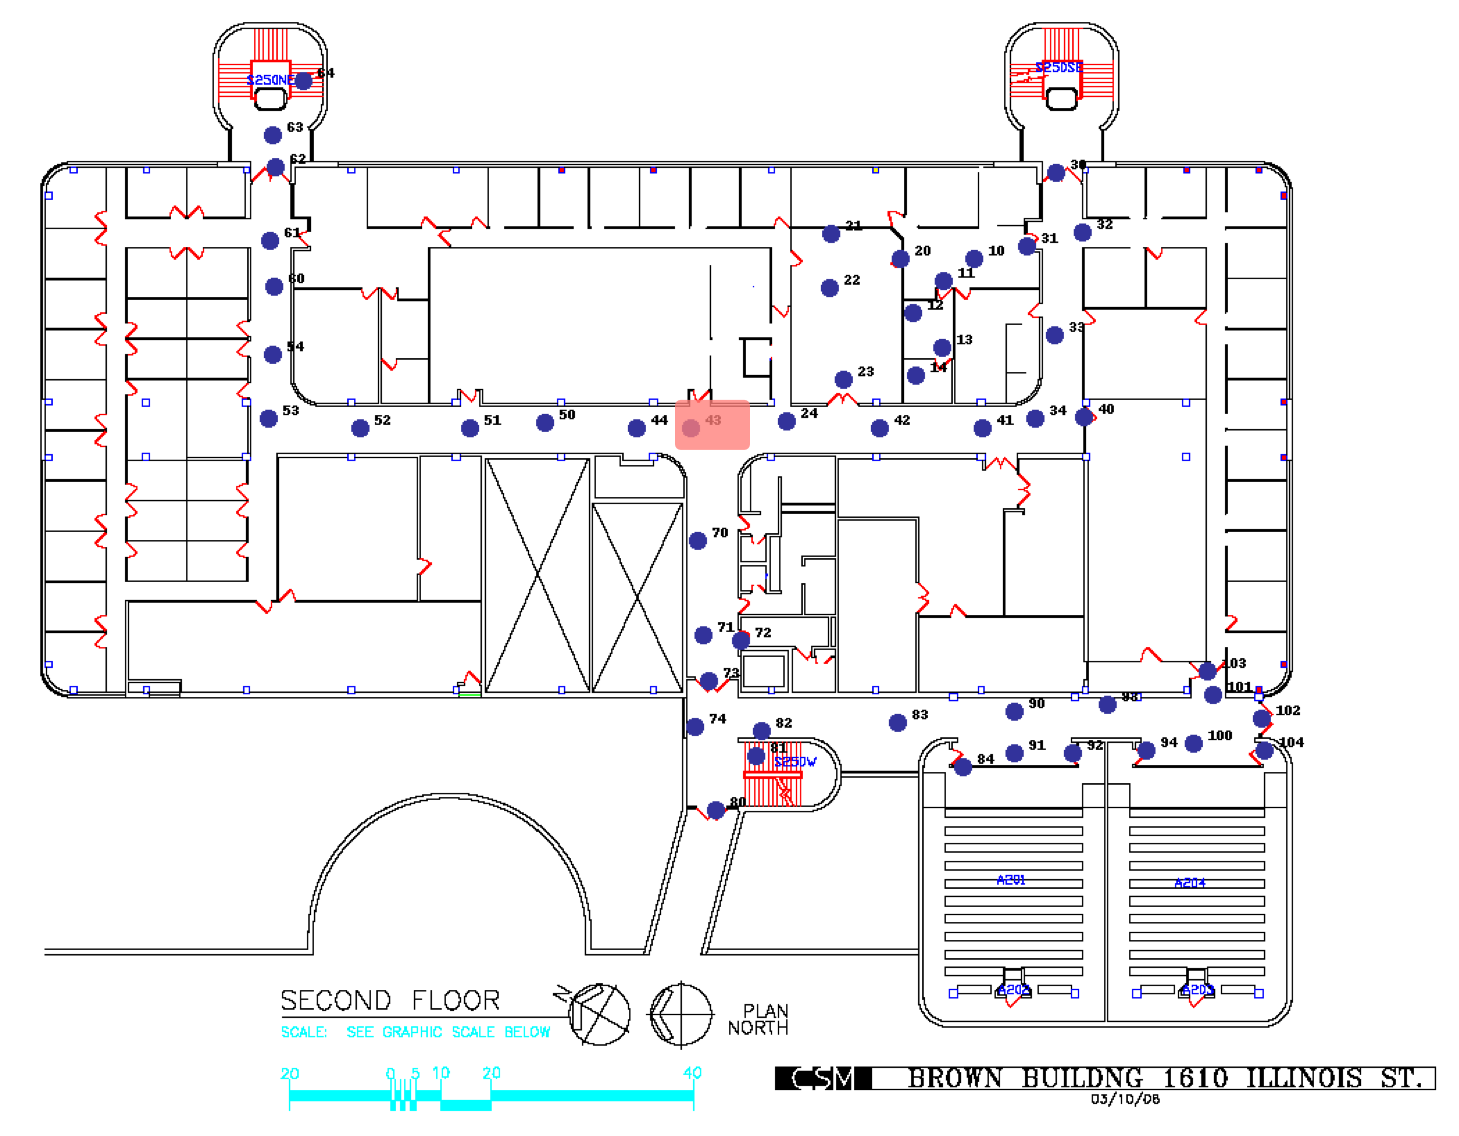
\includegraphics[width=0.5\textwidth]{brown_motes.png}
	\end{center}
	\caption{Sensor locations for the Colorado School of Mines Brown Building}
	\label{fig:csmbbfloor}
\end{figure}

The Colorado School of Mines dataset is a collection of 50 passive infrared sensors mounted on the ceiling of the second floor of a class and office room building.  The density of the sensor placement depends on the location within the building.  Outside the auditorium in the lower right of Figure~\ref{fig:csmbbfloor} is a dense collection of sensors placed approximately every few meters.  Throughout the rest of the building the sensors are placed roughly every 5 meters.  Data was collected for one academic school year from 2008 to 2009 and there are more than 23 million sensor readings.  To acquire readings, the sensors were polled every second and recorded data if motion was detected.  

\begin{figure}[h]
	\begin{center}
		\subfigure[] {
			\includegraphics[width=0.49\textwidth]{brown_day_raw_wed.png}
		}
		\subfigure[] {
			\includegraphics[width=0.49\textwidth]{brown_day_raw_thurs.png}
		}
	\end{center}
	\caption{Average readings from Wednesdays and Thursdays for a given sensor from the MERL dataset.}
	\label{fig:brown_day_raw}
\end{figure}

\ref{fig:brown_day_raw}

This dataset is much different than the MERL dataset as classes typically provide activity on a rigid schedule during the day.  Also as students have exams and projects, late night motion is sporadic based on the time of year.  The counts of sensor activations have been aggregated over every 10 minutes.  Despite occasional late night motion during exam time, most nights have no significant motion.  For this reason we focus on data between 7:00am and 7:00pm daily.  

A plot of the average activations of all Wednesdays and Thursdays for a single sensor along with a range of one standard deviation is given in Figure~\ref{fig:csmday}.  The defined peaks in the dataset correlate to class start and end times when most students will be in the hallways of the building.  Notice how the peak times differ from Wednesday to Thursday.  Classes at the school typically fall into two different schedules; either a class meets on Monday, Wednesday and Friday where the classes are 50 minutes in length or a class meets on Tuesday and Thursday where the classes are 75 minutes in length. 

\begin{figure}[!ht]
	\begin{center}
		\subfigure[] {
			\includegraphics[width=0.45\textwidth]{brown_aggregate.png}
		}
		\label{fig:brown_scaled_aggregate}
		\subfigure[] {
			\includegraphics[width=0.45\textwidth]{brown_oneDay.png}
		}
		\label{fig:brown_scaled_raw}
	\end{center}
	\caption{Scaled average readings for a given day and scaled readings for two days from the CSMBB dataset.}
%	\label{fig:merl_scaled}
\end{figure}

For this work, we focus on the Monday, Wednesday and Friday class schedules.  Figure ~\ref{fig:brown_scaled_aggregate} shows the average of our CSMBB dataset.  Figure ~\ref{fig:brown_scaled_raw} shows a example of raw sensor activations for two days within our CSMBB dataset.


\subsection{Traffic datasets}
Numerous traffic datasets have been used in the time series forecasting literature \cite{Kamarianakis2003, Smith2002, Williams2003, Zhang2009}.  Vehicular traffic datasets are an excellent test for forecasting algorithms as they tend to be highly repetitive with a significant seasonal component.  

\begin{figure}[t!]
	\begin{center}
		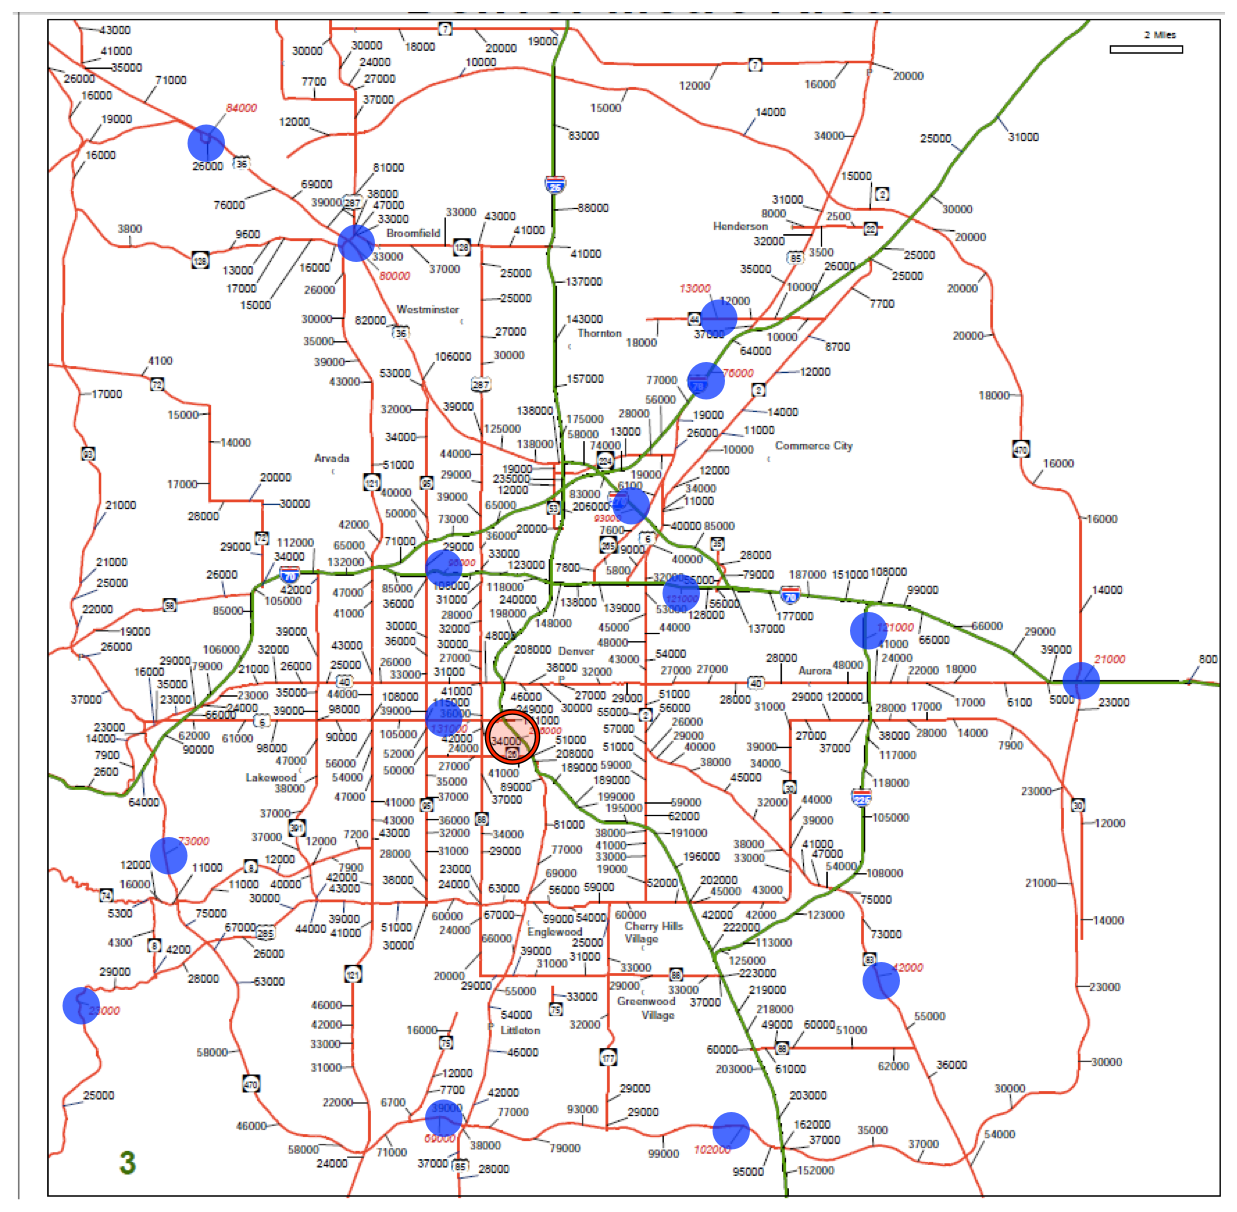
\includegraphics[width=0.5\textwidth]{denver_sensors.png}
	\end{center}
	\caption{City of Denver traffic sensors.}
	\label{fig:denvertraffic}
\end{figure}


\subsubsection{Denver traffic dataset}
The Denver traffic dataset is collected from many in road (TODO FIGURE OUT SENSOR TYPE) sensors which count the number of vehicles passing the sensor throughout the day.  Data is available from 2008 to 2011 on most days of the week.  The data is nearly 1 million readings for the sensors we extracted and approximately 33,000 readings for any one sensor.  For this work we use a freeway sensor near downtown Denver, closely located to Mile High Stadium; the home of the Denver Broncos.  The sensor is located on figure ~\ref{fig:denvertraffic} represented by a red rectangle.

\begin{figure}[h]
	\begin{center}
		\subfigure[] {
			\includegraphics[width=0.49\textwidth]{denver_day_raw_sun.png}
		}
		\subfigure[] {
			\includegraphics[width=0.49\textwidth]{denver_day_raw_mon.png}
		}
	\end{center}
	\caption{Average readings from Sunday and Monday for a given sensor from the Denver traffic dataset.}
	\label{fig:denver_day_raw}
\end{figure}

Count data is aggregated per hour for each direction of traffic at every sensor location.  This data is highly repetitive as Monday through Thursday have approximately the same daily traffic patterns.  Friday behaves much like the rest of the weekdays with the differences being that evening rush hour happens about an hour earlier and their is an increase in night activity.   Example averages for a Sunday and Monday are represented in figure ~\ref{fig:denver_day_raw}.  This figure clearly shows how Monday has a peak time during morning rush hour and a small peak again during afternoon rush hour.  Sunday shows no such pattern.  Instead Sunday shows more slow increase in activity throughout the day.  Also of note is the large amount of sensor activations per hour compared to the CSMBB and MERL datasets.  The counts for Denver traffic are thousands of times larger than our building datasets.

\begin{figure}[h]
	\begin{center}
		\subfigure[] {
			\includegraphics[width=0.45\textwidth]{denver_aggregate.png}
		}
		\label{fig:denver_scaled_aggregate}
		\subfigure[] {
			\includegraphics[width=0.45\textwidth]{denver_oneDay.png}
		}
		\label{fig:denver_scaled_raw}
	\end{center}
	\caption{Scaled average readings for a given day and scaled readings for two days from the Denver traffic dataset.}
%	\label{fig:merl_scaled}
\end{figure}

The scaled dataset that we use for this work is shown in figure \ref{fig:denver_scaled_aggregate}.  This is an average of all Monday through Thursdays for the sensor indicated earlier.  Also, unlike in the other datasets, we do not cut the data down to specific times of day.  This is done, both because there is more traffic during the early morning and late night on this dataset compared to the others and because the data is aggregated only every Hour, do not want to remove more reading from the dataset.  Finally figure \ref{fig:denver_scaled_raw} shows an example of two days of scaled data.  Due to the one hour readings instead of 10 minute readings, the data appears much smoother.  

\subsection{Additional notes on the datasets} 

\noindent
\textbf{Variation in datasets} \\
These three datasets are distinct in many ways.  They differ significantly in total volume of sensor activations, levels of noise in the systems and types of patterns within the datasets.  We believe this variation sufficient to demonstrate the efficacy of our approach to forecasting time series for human controlled environments. \\

\noindent
\textbf{One sensor vs Multiple sensors - why we use a univariate dataset} \\
For this work, we use only one sensor to perform our forecasts.  While intuition may imply that a multivariate approach to forecasting out perform a univariate approach this was show to not be the case by Kamarianakis and Prastacos \ref{kamarianakis2003}.  They studied the problem of forecasting vehicular traffic flow and found similar results using both multivariate and univariate approaches.

We believe the same results hold when it comes to building datasets instead of vehicle datasets.  This is primarily motivated by the simple fact time aggregation and building scale.  For our building datasets, the data is accumulated in 10 minute intervals.  That resolution of detail was empirically selected because it smooths the data sufficiently to allow for accurate forecasting while still being short enough to provide meaningful forecasts.  10 minutes is however, long that it takes an individual to walk from one end of our buildings to the other.  Therefore at a scale of 10 minutes, knowledge of occupancy in one sensor does not seem to imply occupancy in another sensor. \\

\noindent
\textbf{Missing values in the dataset} \\
Due to data collection problems with sensors, the raw data from all of our datasets all had segments with missing values.  These missing values were replace with the historic average value for that sensor at that time on that day.  For example a missing value at 3pm on a Tuesday in the Denver dataset would be replaced by the average value of all Tuesdays at 3pm.






\chapter{BUILDING A NEW ENSEMBLE FORECASTER - IMPROVED LONG TERM FORECASTING}
\label{ch:BCF}
A short discussion on the various approaches and why we consider this approach to lead to better long term traffic forecasts.  Perhaps discuss the typical drawbacks of ensemble approaches and finally discuss how we plan to address those drawbacks here.

This rest of this chapter derives the BCF approach for readers unfamiliar with it and then describes some modifications of the approach which improves its performance for our application.

TODO
\begin{itemize}
	\item Change notation to be in line with our earlier notation.
	\item Write at least one todo item per half day at work.

\end{itemize}

\subsection{Why ensemble forecasting?}
\begin{figure*}[t]
\centering
\includegraphics[width = .55\linewidth]{svm_standard_deviations_vs_horizon.png}
\caption{Standard deviation of support vector machine residuals for all Wednesdays in MERL dataset.  Time index represents 10 minute intervals from 6:00am to 7:00pm.}
\label{fig:svmstd}
\end{figure*}

\ref{fig:svmstd}


\subsection{Bayesian Combined Forecasting}
The BCF approach \cite{Petridis2001} is one of several types of methods which attempt to combine other forecasting models for time series. We selected this forecasting method over other multiple model forecasting methods (such as mixture of experts or ensembles of neural networks) due to its modularity and strong statistical backing.  BCF is modular in that it allows for the component forecasting models to come from any trained forecaster with a well defined distribution of the forecaster's mis-forecasts.  Its statistical backing comes from its direct derivation from Bayes' rule.

\subsection{Bayesian Combined Forecasting Derivation}
To derive BCF we first assume the existence of $K$ models.  From these $K$ models, we want to create a probability distribution on a new random variable $z$ that is used to determine if model $k$ is the correct model from which to forecast at time $t$.  To do this we use the notation of Petridis \cite{Petridis2001} and define $p_{t}^{k}$ as follows
\begin{equation}
p_{t}^{k} = p(z = k | T_{t}, ..., T_{1}).
\end{equation}

From here we apply Bayes rule and get
\begin{equation}
p_{t}^{k} = \frac{p(T_{t} | z = k, T_{t - 1}, ..., T_{1}) \cdot p(z = k | T_{t - 1}, ..., T_{1})} {p(T_{t}, ..., T_{1})}.
\end{equation}
\noindent
Notice that $p(z = k | T_{t - 1}, ..., T_{1}) = p_{t - 1}^{k}$.  Thus we can create a recursive estimation based on prior $p_{t}^{k}$.

With recursive values for $p_{t}^{k}$ and replacing $p(T_{t}, ..., T_{1})$ with a conditional probability on $z$ we get
\begin{equation}
p_{t}^{k} = \frac{p(T_{t} | z = k, T_{t - 1}, ..., T_{1}) \cdot p_{t - 1}^{k}} {\sum_{j = 1}^{K}p(T_{t} | z = j, T_{t - 1}, ..., T_{1}) \cdot p_{t - 1}^{j}}.
\end{equation}

We use the empirically observed forecasting error for each model to estimate $p(T_{t}|z = k, T_{t - 1}, ..., T_{1})$.  The forecasting error for a given model at time $t$ is 
\begin{equation}
e_{t}^{k} = \bar{T}_{t}^{k} - T_{t}.
\end{equation}
\noindent
We can use these forecasting errors to estimate a probability distribution for each model on the random variable $e_{t}^{k}$.  This is typically modeled as a white noise zero mean Gaussian process.  For our work, we represent this as a distribution of error terms with some parameterization $\omega_{k}$.  Thus for each model the probability error distribution function on the model error random variable is given by $q(e_{t}^{k};\omega_{k})$.

The final equation for the posterior probability of a given model $k$ is
\begin{equation}
\label{eq:model_prob}
p_{t}^{k} = p(z = k|T_{t}, ..., T_{1}) = \frac{p_{t - 1}^{K} \cdot q(T_{t} - \bar{T}_{t}^{k}; \omega_{k})}{\sum_{j=1}^{K}p_{t - 1}^{j} \cdot q(T_{t}^{j} - \bar{T}_{t}^{j}; \omega_{j})}.
\end{equation}

An example of these changing normalized posterior probabilities for a small section of the MERL dataset is shown in Figure~\ref{fig:probsmerl}.

Forecasting using BCF is done by either computing a weighted forecast $\delta$ time steps into the future for each forecasting model or by simply selecting the model with the highest likelihood.  For this paper we forecast using a weighted forecast of all models.  The forecasting equation is
\begin{equation}
T_{t + \delta}^{ALL} = \sum_{k=1}^{K}p_{t}^{k} \cdot \bar{T}_{t + \delta}^{k}.
\end{equation}

\begin{figure}
\centering
\includegraphics[width = 1.0\linewidth]{posterior_probs.png}
\caption{Normalized posterior probabilities of component models on a section of MERL dataset.}
\label{fig:probsmerl}
\end{figure}

\subsection{BCF Modifications}
In this subsection we discuss a number of modifications to maximize the effectiveness of BCF for our data.  We refer to the modified BCF algorithm as Bayesian Combined Forecasting for multiple Time Steps or BCF-TS for short.  These modifications  enable BCF to work with forecasting horizons greater than one in the future.

\subsubsection{Forecast $\delta$ time steps into the future}
Traditional implementations of BCF in other domains \cite{Petridis2001, Zheng2006} are interested only in 1 time step ahead forecasts.  For our work we require forecasts that are $\delta$ steps ahead which requires a small change to the BCF method.  Instead of generating a model's error distribution from 
\begin{equation}
e^{t}_{k} = \bar{T}_{t}^{k} - T_{t} = f(\bar{T}_{t},T_{t - 1} ..., T_{1}; \theta_{k}) - T_{t}.
\end{equation}

The error distribution is instead generated from 
\begin{equation}
e^{t}_{k} = f(\bar{T}_{t}, ..., \bar{T}_{t - \delta + 1}, T_{t - \delta}, ..., T_{1};\theta_{k}) - T_{t}.
\end{equation}
The reason for this change is due to the assumption that our error distribution is an accurate representation forecasting accuracy.  
The forecasting error distribution for models at $1$ time step into the future is not necessarily the same as models at $\delta$ time steps.  Thus we compute a different error distribution for each forecast time step.


\subsubsection{Improving model error distributions}
Despite other implementations of BCF using fixed error distributions, our data has clear daily trends.  For some of our models, the forecasted residuals follow these same trends.  See Figure~\ref{fig:svmstd} for an example of how the forecasting error distribution for a trained support vector regression model on the MERL dataset depends on the time and on the forecasting horizon.

To represent a more realistic error distribution instead of a fixed white noise Gaussian that is commonly used in the literature, we fit a Gaussian for each 10 minute slice of a given day.  The data from the MERL dataset was used from 6:00am to 7:00pm. The thirteen hours of data used per day represent 78 time slices.  For example taking the data for each time slice for each Wednesday results in 78 Gaussian error distributions for each forecasting horizon.  These Gaussians are computed from a validation set representing 20\% of our data.  It is from this set of models error distributions that we compute BCF.

As a possible improvement to this set of error distributions, we note that using a generalized autoregressive conditional heteroskedastic (GARCH) model \cite{Box2008} or some other appropriate model to forecast future variance based on local and historic changes in variance would likely outperform our time based average Gaussian models.  GARCH models are similar to seasonal autoregressive moving average models which we use as one of our component forecasting models.

\subsubsection{Model selection thresholding}
Diebold \cite{Diebold1991} cautions against the use of forecasting using a Bayesian combination of models in all cases.  Diebold points out that under certain situations a convex combination of forecasts for models may not be optimal, and cases exist where taking negative likelihood weighting may be optimal.  These conditions are likely to arise during instances where the data may not be accurately described by any of the forecasting models.  

Furthermore when such cases where no model is able to provide an accurate forecast, then it is often the case that forecasts come from the worst model.  

To combat this case, we have implemented a model selection threshold $h_{k}$.  If the likelihood of all component models is below $h_{k}$, then we forecast from only the model which is historically the most accurate based on our validation set.  

The threshold is different for each model, and should depend on the error distribution of the model.  In practice we have found that $2\sigma$ serves as a good threshold.  Basing the threshold on $\sigma$ is useful as it provides a threshold value which does not depend on $e^{k}_{t}$.  For a zero mean Gaussian the probability of the $2\sigma$ threshold is
\begin{equation}
p(2\sigma) = \frac{1}{\sigma\sqrt{2\pi}}e^{-2}.
\end{equation}
Because the Bayesian combined forecasting approach is iterative, it is possible that a long section of forecasts that indicate one model correct or incorrect can lead to likelihood underflow.  Due to this problem we adjust our normalized likelihoods so that no model may reach a value below 0.001.  This empirically chosen value is low enough to not have a great impact on forecasts while still being high enough to allow model likelihoods to change quickly.

\subsection{Results of Ensemble}

BCF and BCF-TS (BCF with our specific set of modifications) were trained and tested using all component models described above.  All of the models were trained on 60\% of the total datasets.  Another 20\% was used for model validation and the final 20\% used for testing.  All results shown below are on the test set only.  Figure~\ref{fig:realbcf} shows an sample section of test data from the MERL dataset along with BCF-TS forecasts for horizons of 1 and 5.   As expected as the forecasting horizon increases the forecasts become less accurate.

\begin{figure}[h]
\centering
\includegraphics[width = 1.0\linewidth]{real_forecasts_bcf.png}
\caption{A comparison of forecasts at various horizons against real data for an sample time segment using BCF-TS.}
\label{fig:realbcf}
\end{figure}

It is common for one model's normalized posterior probability to be near one when that model is currently accurate.  Figure~\ref{fig:realbcfsvm} shows as example of this behavior.  From time index 1 to 8, the SVM component model has a posterior probability near 1.0 and as a result BCF-TS forecasts nearly completely from this model.  Then from time index 9 on the model's posterior probability is lower and as a result BCF-TS uses other model for its combined forecast.

\begin{figure}[h]
\centering
\includegraphics[width = 1.0\linewidth]{real_forecasts_bcf_svm.png}
\caption{A comparison of BCF-TS and SVM forecasts at horizon equal to three against real data.}
\label{fig:realbcfsvm}
\end{figure}

Figure~\ref{fig:rmseplot} shows the results of the root mean squared error (RMSE) of forecasts across a forecast horizon up to 10 time steps (100 minutes) into the future for each model.  These plots show that BCF-TS has the lowest error.  However, the average model shows itself to be a strong indicator of future activity for forecasts beyond 60 minutes into the future.  Forecasts were performed for significantly longer horizons, but the results were uninteresting as the total RMSE of models converged to roughly the values at a forecasting horizon of 10 time steps.  

\begin{table}
\centering
\caption{Run times (in seconds) for each forecasting horizon.}
\begin{tabular}{|c|c|c|c|c|c|c|c|} \hline
Algorithm & $1$ & $2$ & $3$ & $5$ & $8$ & $10$ \\ \hline
Average & 0.001 & 0.001 & 0.001 & 0.001 & 0.001 & 0.001 \\ \hline
ARIMA & 0.043 & 0.045 & 0.046 & 0.053 & 0.058 & 0.063\\ \hline
SVM & 0.048 & 0.910 & 0.137 & 0.227 & 0.357 & 0.444 \\ \hline
TDNN & 20.87 & 21.60 & 21.82 & 21.28 & 22.73 & 22.50 \\ \hline
BCF-TS & 20.97 & 21.26 & 21.27 & 21.34 & 21.57 & 21.63\\ \hline
\end{tabular}
\label{fig:runtimestab}
\end{table}

In the CSMBB dataset the Seasonal ARIMA model was a good forecaster of future activity while in the MERL set it performed significantly worse than even the average model on all forecasting horizons.  This is likely due to a stronger seasonal component to the CSMBB dataset due class schedules.  Instead on the MERL dataset there is little seasonal correlation and thus natural variance from a prior season may incorrectly affect current forecasts.  This result is similar to that of other papers that use seasonal ARIMA models \cite{Newsham2010}; where in the case of strong seasonal data, results are better for short horizon forecasts, but longer forecasts favor historic averages.

BCF and BCF-TS were both better at a horizon of one time step for all component models (see Table~\ref{fig:rmsetab}).  In the MERL dataset standard BCF was outperformed by SVM and later the average model for all forecast beyond one horizon.  However the BCF-TS model showed significant improvement in RMSE scores for all forecasting horizons unto 60 minutes.  For horizons of 10 time steps and greater, the average model is about as good as the BCF-TS approach.

Table~\ref{fig:runtimestab} shows the run time in seconds of each forecasting algorithm at a given forecasting horizon.  The times are for forecasting the entire test set on the MERL dataset for a single sensor, approximately twenty weeks worth of data.  In general BCF-TS was slower than any component model, but the times are still such that real-time forecasting is possible.

\begin{figure}[!ht]
	\begin{center}
		\subfigure[] {
			\includegraphics[width=0.49\linewidth]{brown_rmse.png}
			%\caption{CSMBB forecasting model errors}
			%\label{fig:csmrmse}
		}
		\subfigure[] {
			\includegraphics[width=0.49\linewidth]{merl_rmse.png}
			%\caption{MERL forecasting model errors}
			%\label{fig:merlrmse}
		}
	\end{center}
	\caption{Root mean square error of forecasting for each model vs forecasting horizon.}
	\label{fig:rmseplot}
\end{figure}




\chapter{ACTIVITY RECOGNITION ENSEMBLE FORECASTING}
In the past chapter, we showed that a few changes can lead to some significant improvements in multi-step forecasting accuracy when ensemble Bayesian combined forecasting is applied to our traffic datasets.  This chapter initially investigates BCF further by exposing some potential problem scenarios.  We look at some related work into potentially solving these problems through the identification and modeling of activities and finally introduce a new ensemble forecasting technique which solves many of these problems.  

\begin{figure}[!b]
	\begin{center}
		\subfigure[] {
			\includegraphics[width=0.49\textwidth]{sample_residual_event_804.png}
		}
		\subfigure[] {
			\includegraphics[width=0.49\textwidth]{sample_residual_event_6024.png}
		}
	\end{center}
	\caption{Two similar events occurring at different time in the same Denver residual dataset.}
	\label{fig:sample_residual_events}
\end{figure}


%%%%%%%%%%%%%%%%%%%%%%%%%%%%%%%%%%%%%%%%%%%%%%%%%
%Need for another ensemble forecaster
%%%%%%%%%%%%%%%%%%%%%%%%%%%%%%%%%%%%%%%%%%%%%%%%%
\subsection{The need for another ensemble forecaster}
When analyzing the residual datasets of these ensemble forecasts, we noticed a fundamental problem with our forecaster.  In the residual forecasts of BCF and many of the forecasting algorithms, the resulting residual forecast would still have many repeated misforecasts that could not be explained by random noise.  As alluded to in Chapter 1, these repetitive misforecasts may come from large human controlled scheduled events (such as sporting events, public celebrations, or in the case of buildings - meetings) or they may be from uncontrolled and unscheduled events (such as weather or traffic accidents).  

\begin{figure}[!t]
	\begin{center}
		\subfigure[] {
			\includegraphics[width=0.49\textwidth]{denver_bcf_residual_15.png}
		}
		\subfigure[] {
			\includegraphics[width=0.49\textwidth]{denver_bcf_residual_26.png}
		} \\
		\subfigure[] {
			\includegraphics[width=0.49\textwidth]{denver_bcf_residual_32.png}
		}
		\subfigure[] {
			\includegraphics[width=0.49\textwidth]{denver_bcf_residual_38.png}
		}
	\end{center}
	\caption{Scaled histogram of IBCF residual values for the Denver traffic dataset at various daily time steps.  The red line is the corresponding best fit Normal distribution.  Notice how in all plots there exist data points which exist after the tails of the Normal distributions have approached zero.}
	\label{fig:denver_bcf_residual}
\end{figure}

\ref{fig:sample_residual_events} shows two of these events occurring.  Such an event clearly occurs outside the normal behavior noise of our data.  The light red region in this image represents the one standard deviation boundary for the residual data.  From Chapter 4, we know that BCF residual data tends to be normally distributed per daily time step.  The residual datasets from each time step pass the one-sample Kolmogorov-Smirnov \cite{Marsaglia2003, Lopes2007} test for normality ($p \ge 0.1$).  Assuming this data is truly normally distributed then the odds of getting even one such datapoint outside the $\pm 3 \sigma$ should occur roughly 1 in every million data points.  Yet, in our Denver traffic data, we had 22 such instances in the testing dataset alone ($N \approx 12000$).  

\ref{fig:denver_bcf_residual} the distribution of our datasets graphically.  In this figure, a histogram of the data from four different fixed daily time steps from the Denver traffic dataset, overlaid with the corresponding best fit normal distribution.  In each image the same pattern appears.  Residual values around the mean and on the tails tend to occur with a greater frequency than would be suggested by a normal distribution.  Values around the mean are not the problem.  These values correspond to accurate forecasts.  Values around the tail however are problematic and are further evidence of large events being one of the causes of noise in our residual data.

The unlikely existence of these tail events combined with evidence that the overall residual time series behaves as a white noise Gaussian process provides evidence that these events are likely not due to natural noise and instead due to other factors.  The remainder of this chapter discusses ways to identify and model these anomalous events along with providing an algorithm for using these events to improve our forecasting algorithm.


%%%%%%%%%%%%%%%%%%%%%%%%%%%%%%%%%%%%%%%%%%%%%%%%%
%Overview ABCF
%%%%%%%%%%%%%%%%%%%%%%%%%%%%%%%%%%%%%%%%%%%%%%%%%
\subsection{Bayesian combined forecasting with activity and anomaly modeling (ABCF)}

\begin{wrapfigure}{L}{0.3\textwidth}
\centering
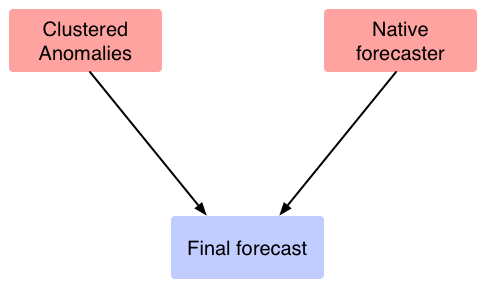
\includegraphics[width=0.25\textwidth]{simple_approach_overview.png}
\caption{Extremely high level overview of our approach}
\label{fig:highlevel_overview}
\end{wrapfigure}

As outlined in the introduction, we return here to a brief discussion of our approach.  The structure of non-Gaussian anomalies in the residual datasets of our forecasts leads us to explore if models of these anomalies can be used to improve our forecasts.  We propose a hybrid ensemble approach which can be applied to any forecaster and may lead to improved results.  

A high level view of our approach is detailed in \ref{fig:highlevel_overview}.  Given any trained forecaster, we extract a set of residual data.  Searching this residual dataset, we next attempt to extract and model the most representative set of anomalous events.  From \ref{fig:sample_residual_events}, we know that for our traffic systems - and we believe for many other traffic systems with repeated events - these events are not unique and are likely to repeat with similar behavior.  These anomalous events are then used as the basis of an ensemble forecaster combined with a zero mean background model which represents the native forecaster.  

In Section \ref{sec:abcf} we introduce a recursive ensemble forecaster which uses clustered anomalies as inputs and works on the residual dataset of any given native forecaster.  Finally, using both the anomaly ensemble inputs and the native forecast, we combine the results to produce a final forecast.  


%%%%%%%%%%%%%%%%%%%%%%%%%%%%%%%%%%%%%%%%%%%%%%%%%
%Background literature
%%%%%%%%%%%%%%%%%%%%%%%%%%%%%%%%%%%%%%%%%%%%%%%%%
\subsection{Background literature on activity recognition and anomaly detection}
To construct our approach we need to identify and model these anomalous events.  Considerable work has been done in the field of time series anomaly detection; however this work is typically limited to anomaly detection and classification.  We were unable to find many academic references using anomaly modeling techniques for improved forecasting.  We believe that this limited amount of anomaly modeling work is due to the nature of anomalies; either they are random and difficult to predict as is the case with stock market anomalies ~\cite{Kontonikas2013, Thushara2014} or they require some immediate attention and thus forecasting is an inappropriate response to the anomaly.  Such a situation arises frequently in network data monitoring.  Detection and classification of network anomalies help to determine potential network attacks \cite{Tartakovsky2013, Gogoi2011} and allow for preventive measures to take place, but forecasting network traffic during these anomalies is of little utility.  
   
Our anomalies tend to be repetitive and multiple time steps in length.  Data of this form is very closely related to another field of time series data analysis - that of activity recognition.   Due to the broad nature of this term and the breadth of research on anomaly detection, we briefly discuss some of the ways in which time series anomaly detection and activity recognition has been utilized in the past as a way to familiarize the reader with a discussion of the literature.  This review is not meant to be a complete list of all works in these fields, but instead gives an overview of the types of work done in this field so that we may better contrast previous work with our approach.

\bigskip
\noindent \textbf{Anomaly Detection} \\
From Eamon Keogh, a prominent researcher in time-series anomaly detection, a reading or series of readings is anomalous in a time-series if the 

\begin{quote}
"frequency of occurrences differed substantially from that expected, given previously seen data. \cite{Keogh2002}"
\end{quote}

A common method of anomaly detection is through the use of tools to assist in visual identification \cite{Stoffel2013, Lakhina2004, Shi2012}.  Tools have been extensively developed for network anomaly detection.  Such tools allow network administrators and researchers to quickly identify and potentially classify anomalies in the form of certain network attacks.  This is done by giving providing graphs, and overlay visualizations which make the identification of patterns more apparent.  Through the use of these tools, network administrators are able to quickly respond to  various attacks and minimize the potential damage to the network.  Visual assistance tools for anomaly detection do not provide modeling and forecasting of anomalies and thus are of little utility for utilizing anomalies to improve traffic system forecasting.   

Another common technique for anomaly detection within time series data is known as change point (or step detection).  Originally developed for statistical quality control, the cumulative sum control chart (CUSUM) \cite{page1955} is a classic algorithm for detecting changes in the mean of a time series.  It involves the calculation of a cumulative sum of the weighted observations.  When this sum exceeds a certain threshold value, a change in value is declared. 

The field of change point detection is quite heavily researched.  Researchers have developed algorithms for most types of data and computational scenarios.  There are algorithms to detect changes in time series mean, changes in variance and changes in distribution from the exponential family \cite{Dessein2013}.  These algorithms can operate offline, online \cite{Tartakovsky2013}, top down, bottom up and globally.  Excellent summaries of current state of the art in change point detection spanning all major formulations (Bayesian, minimax, and generalized Bayesian) are found in \cite{Polunchenko2012, Reeves2007}.  

For some time after the original CUSUM change point method, research moved to more parametric stochastic models.  Researchers would look for statistical changes in a time series that fit another distribution or family of distributions, for example Adams and MacKay's paper on Bayesian Online Change Point Detection \cite{Adams2007}.  Such methods are powerful when the change point distributions are known a priori, however we do not assume such knowledge.  

Another more recent paper from Liu et al. \cite{Liu2013} discusses an entirely different change point detection technique which relies on the ratio between the distribution of some samples at time $t$ and some further samples at time $t + n$.  Through ratio estimation, researchers can use a dissimilarity measurement on non parametric models of the data to estimate change points.  The power of this technique comes from directly estimation the ratio of probability densities and not the densities themselves.  From this density estimation, the rational is that knowledge of the two densities implies the ratio, but the ratio does not uniquely imply the densities and thus the ratio may be easier to estimate while still giving knowledge of the change point.  

The problem with general change point techniques for our data is that our data distributions change constantly throughout the day.  Our MERL dataset shows large amounts of activity during lunch time and work start and end times.  We are interested in those instances where activities are anomalous.  Our technique uses a combination of peak finding and time of day residual CUSUM.  A detailed description of our technique and results will be shown later.

\bigskip
\noindent \textbf{Individual Activity Modeling and Recognition} \\
Work in activity recognition has focused on recognizing either individual activities or group activities.  In this section we describe many of the individual activity recognition techniques.  One common type of individual activity recognition is from wearable sensors such as accelerometers or RFID tag readers.  This type of work is almost always supervised and the goal is to map sensor readings to a comprehensible activity such as dish washing or tooth brushing \cite{Wang2009,Bao2004}.  While some of this has potential applications to our goals, much of it is not applicable as the focus is typically on recognizing activities from fully labeled datasets.  Authors from this field have used many of the standard machine learning models: decision trees \cite{Bao2004}, support vector machines \cite{Krishnan2008,Bao2004,Lustrek2009}, naive Bayes \cite{Bao2004,Lustrek2009}, nearest neighbor \cite{Bao2004,Lustrek2009}, and hidden Markov Models (HMM) \cite{Wang2009,Oliver2002}.  Comparisons amongst models have shown that performance is data dependent and that no one model appears to be best for all types of activities \cite{Bao2004,Lustrek2009}

Huynh \cite{Huynh2008} used a naive Bayes classifier in a different way for wearable sensor individual activity recognition.  Instead of using it to describe activity, it was used as a dimensionality reduction technique; the results of which were the basis for a dictionary in latent Dirichlet allocation \cite{Blei2003}.  The topics generated from latent Dirichlet allocation are then clustered using k-means.  Each of these clusters represents a single activity.  This clustering approach proved effective for the recognition of repeated activities throughout the day, but due to its reliance of a fixed ratio of latent Dirichlet allocation projected topics, it is likely that recognizing combinations of activities will prove problematic.

To account for activities of varying time lengths, probabilistic suffix trees \cite{Hamid2007} have shown to be an effective model for activities.  Trees are trained using all sequential subsets of an input sequence and a total model is then created from the set of trees using AdaBoost \cite{Freund1996}.  The performance level of suffix trees seems to be highly noise dependent.  \cite{Hamid2006} compared HMMs with suffix trees and found that suffix trees out performed HMMs when the data was without noise, but as the noise increased HMMs performed increasingly better, eventually surpassing the performance of suffix trees.

\bigskip
\noindent \textbf{Group Activity Modeling and Recognition} \\
There are a limited number of publications that exist on group activity modeling recognition using a large number of sensors.  Within this problem domain the challenges to solve are different due to the type of data collected and due to group activities typically occurring over multiple sensors.  The work within this domain that is most similar to our work is from Mitsubishi Electronic Research Laboratories (the creators of the MERL dataset) \cite{Wren2003, Wren2006a}.  The goal of such group activity work is to utilize a set of sensors to describe activities or events which effect many individuals within the environment.  As expected, these group event models are typically used to describe larger or longer movements within the environment.  For example, such modeled events may be holiday movement vs workday movement or general flow through out a building based on sensor topology \cite{Wren2006, Hoff2009}.  
	
HMMs have been used as a model for learned activities.  These models are used to build a tree \cite{Minnen2004, Wren2006a} with each level described by a model with a different number of hidden nodes, meaning that model accuracy is roughly correlated to tree depth.  At the top of the tree are simple models used to describe gross activities.  The leaves of the tree are highly complex models describing specific activities.  This tree structure has the advantage of being computationally efficient while maintaining accuracy on par with other techniques based on clustering of HMMs \cite{Clarkson1999}.  
	
In a method similar to the HMM tree, work has been done to create a hierarchy of fixed filters based on possible sensor topologies \cite{Wren2006}.  At each level of the hierarchy, the number of sensors and the amount of time history increases.  The probability of occurrence of each fixed arrangement is then computed when all levels are created, the resulting model represents the total classifier.  The usage of fixed sensor topologies is highly environment dependent and the fixed time lengths with each level of the hierarchy are likely too restraining for the types of activities we expect to observe.  

From the results of all activity recognition papers, it appears that approaches which show the most promise tend to use a model which allows comparison of inputs with various time lengths.  Also, hierarchical techniques tend to perform better than multiple models of equal complexity.  In defense of these general observations is the work of Huynh \cite{Huynh2005} who found that empirically for his problem, there is not a single feature or time window of past history that will perform best for all activities.  Instead each activity is best modeled by a set of features and length of time unique to that activity.  Huynh postulates that his finding is true of most activity recognition problems.  Our approach, which will be described in detail in the next section is to represent activities as a mixture of Gaussians.  While for this work we use fixed length activities, our ensemble forecaster (described in Section 5.7) is derived to work with activities each which may have any length independent of the other modeled activities.  Modeling mixed length activities is recommended for future work.

\subsection{Anomaly extraction and representation}
As we showed earlier in this section with ~\ref{fig:denver_bcf_residual}, the tails of the best fit Gaussian for the BCF residual random variable tend to have larger than expected likelihoods.  These unlikely residuals do not appear to be completely random.  From a review of the literature, we know that there are numerous methods to extract and model this data.  For our work, we propose a simple extraction technique and then model the data according to a time-series mixture of Gaussians.  This method allows us to impart a probabilistic behavior to our anomaly models.  Such behavior is essential to our eventual forecasting technique.

\begin{figure}[]
	\begin{center}
		\subfigure[] {
			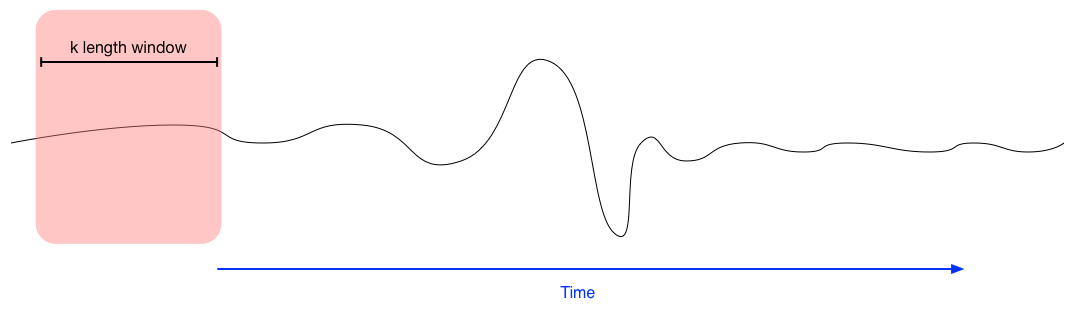
\includegraphics[width=0.50\textwidth]{slide_window_1.png}
		}
		\subfigure[] {
			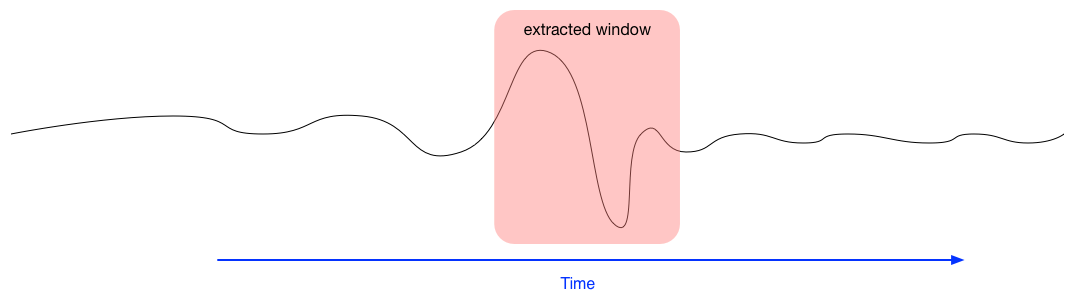
\includegraphics[width=0.50\textwidth]{slide_window_2.png}
		}
	\end{center}
	\caption{Demonstration of a fixed width sliding window looking for locally maximal deviations from background behavior.}
	\label{fig:sliding_window}
\end{figure}

\bigskip
\noindent \textbf{Sliding window data extraction} \\
Given a time series of residual data, we extract the top $k\%$ of the maximum residual data as measured by a fixed length sliding window.  ~\ref{fig:sliding_window} demonstrates visually our method of potential candidate residual data segments to model.  In this example, the fixed length window is slid along a time series and windows with large total residual deviation are selected.  These windows are then centered around the largest peak within the window.  This is done to ensure an easier time clustering as similar extracted residual segments will typically line up with each other.

\begin{algorithm}
	\caption{Algorithm for candidate data extraction}
   	\label{alg:dataextract}
	
	\begin{algorithmic}
		\State \#assume we have access to residual\_data as a one dimensional array
		\State 
		\State extracted\_lengths = []
		\State final\_data = []
   		\State 
				
		\For{$t = 0$; $t <=$ residual\_data.length - window\_width; $t +=$ window\_width}
		\State	window\_sum = sum(abs(residual\_data[$t$:$t +$ window\_width]))
		\State 	extracted\_lengths.append((window\_sum, $t$))
		\EndFor
		
		\State
		\State \#sort the extracted lengths by the window\_sum dimension descending
		\State extracted\_lengths = sort(extracted\_lengths, dim1, order = "descending")
		\State num\_to\_extract = ceil($k$ * extracted\_lengths.length)
		
		\State
		\State \#Center all the extracted residuals by local peaks
		
		\For {$t = 0$; $t < num\_to\_extract$; $t++$}
		\State 	dind = extracted\_lengths[t][1]
		\State	\#Max peak on local window
		\State	mp = find\_max\_peak(abs(residual\_data[dind:dind + window\_width]))
		
		\State
		\State 	\#Recenter the data around the local peak
		\State	final\_data.append(residual\_data[mp - window\_width / 2: mp + window\_width / 2])

		\EndFor

	\end{algorithmic}
\end{algorithm}


Algorithm \ref{alg:dataextract} precisely describes our approach.  The input parameter $k$ is chosen empirically for each dataset and underlying forecasting model.  The effects of this parameter $k$ are discussed later.  A sample of the top 10\% extracted residuals for the MERL dataset is displayed in \ref{fig:extracted_residuals}.

On additional possible technique for data extraction is sparse dictionary coding.  This technique finds a set of primitives (in this case small representations of the time series residual data) which can be used to best approximate the original dataset.  We believe it likely that primitives with the largest residual values would most likely correspond to the anomalies we would like to find.  This technique has been extensively to find primitives activations on time series EMG data \cite{Kim2010} and for image reconstructions \cite{Mairal2009}.  

For this work however, we believe that our constant length anomaly extraction is sufficient to show the strength of our combined forecasting approach.

\begin{figure}
	\begin{center}
		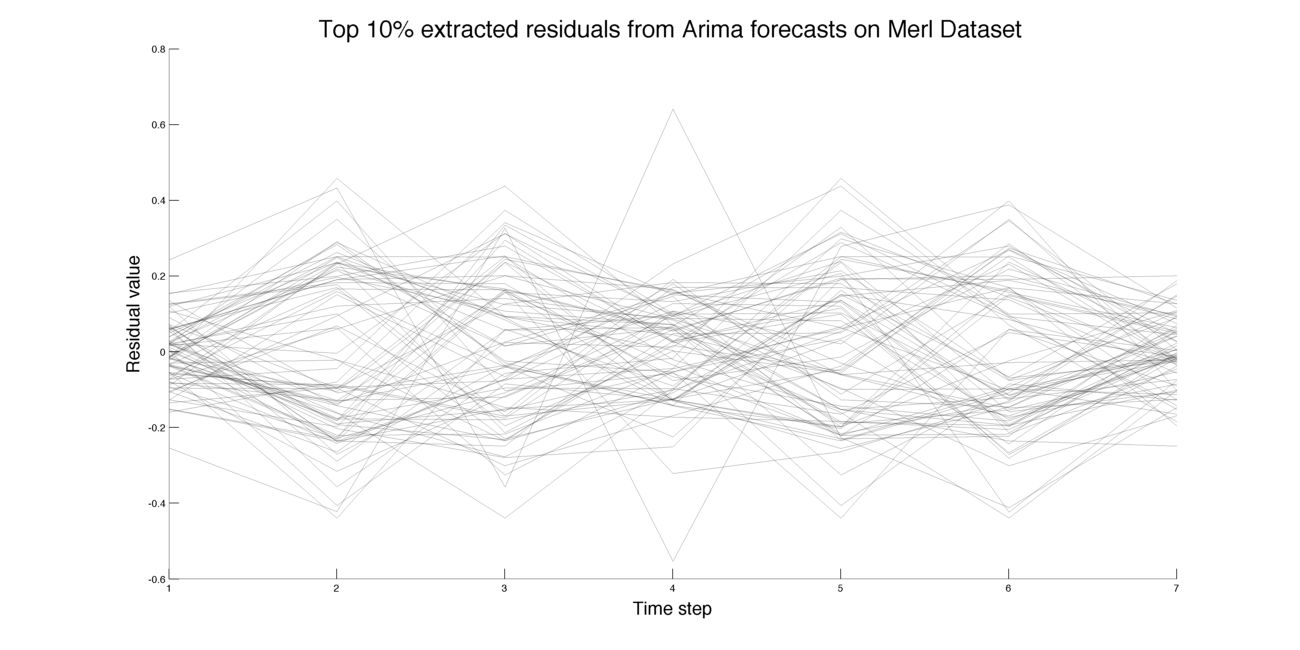
\includegraphics[width=0.90\textwidth]{arima_abcf_extracted_residuals_Merl.png}
	\end{center}
	\caption{Extracted residuals from the MERL dataset using the sliding window extraction method with window length of 7}
	\label{fig:extracted_residuals}
\end{figure}


\subsection{Time series mixture of Gaussians derivation}
A mixture of Gaussians is a strongly supported stochastic data clustering technique used in activity recognition.  This technique models a set of data by positing that each data point ($x_{i}$) is generated from one of $K$ Gaussians.  Borrowing partially the notation of Andrew Ng \cite{Ng2008}, a mixture of Gaussians is described mathematically by specifying a joint distribution $p(x_{i}, z_{i}) = p(x_{i}|z_{i})p(z_{i})$.  $z_{i}$ is multinomial on parameter $\phi$  ($\phi_{j} \ge 0$,  $\sum_{j=1}^{K}{ \phi_{j}} = 1$ and $p(z_{i} = j)$).  Each $x_{i}|z_{i} = j \sim \mathcal{N}(\mu_{j}, \Sigma_{j})$.  From this derivation, the $z_{i}$'s are latent variables which makes the estimation of the Gaussian models more difficult.  The result of mixture of Gaussian training is to produce a soft clustering of every datapoint $x_{i}$ to each trained Gaussian distribution.

Traditionally, a mixture of Gaussians is for data vectors with no time element, but some research has been done on using a mixture of Gaussians for time series data clustering.  In one paper \cite{Eirola2013}, the authors create a design matrix to construct a delayed embedding of the original time series.  Each row in the matrix corresponds to a fixed length vector selected from the input time series.  All of the rows together contain all data from the time series with each row over containing overlapping data with one new time series element.  From this embedding, the authors compute a mixture of Gaussians to approximately reconstruct the time series.  In another paper \cite{Kalliovirta2012} Gaussian mixture models are used to mix the weights of an autoregressive model in an attempt to reconstruct the original time series.

Here we introduce another technique for modeling time series data were we assume the presence of multiple short (typically fewer than 10 time steps) residual time series.  These time series are assumed to be derived from a set of $K$ unique time series.  In each of these time series, we model the time steps as Gaussians, each with their own unique mean and covariance.   For our work, the input time series are those candidate extracted anomalies from the previous section (i.e. we are attempting to model and cluster data from \ref{fig:extracted_residuals}).  The following is our derivation of this approach.

The goal of mixture of Gaussians is to find a set of models which will maximize the log likelihood of the parameters of some models to the dataset.  Given dataset (in this case a dataset of residuals) $\{r^{(i)}\}$ we maximize
\begin{equation}
\ell(\phi, \mu, \Sigma) = \sum_{i = 1}^{M}log\{p(r^{(i)};\phi, \mu, \Sigma)\}
\end{equation}
\noindent 
where ${M}$ is the total number of time series instances.  In this equation, the $r^{(i)}$'s are each time series slices from the candidate residuals.  The $(i)$ represents the $i$th residual candidate time series - we use the $(i)$ notation to distinguish from the exponent operator.  For this work, each $r^{(i)}$ is of fixed length $N$.  $\phi, \mu,$ and $\Sigma$ are the parameters to optimize for each time series Gaussian.  Each $r^{(i)}$ is roughly analogous to $x_{i}$ in the typical derivation of a mixture of gaussians with the difference here that each $r^{(i)}$ is $N$ readings in length.

As in traditional mixture of Gaussians formulation, we introduce a latent variable $z^{(i)}$ which is multinomial on parameter $\phi$ ($\phi_{j} \ge 0$,  $\sum_{j=1}^{K}{ \phi_{j}} = 1$ and $p(z_{i} = j)$).  With this latent variable $z^{(i)}$ we now maximize the likelihood of the joint distribution of $r$ and $z$.  This equation is given as 

\begin{equation}
\ell(\phi, \mu, \Sigma) = \sum_{i = 1}^{M}\log \sum_{k = 1}^{K}p(r^{(i)}, z^{(i)} = k;\phi, \mu, \Sigma)
\end{equation}

In the traditional mixture of Gaussians algorithm each model is ostensibly a Gaussian which may be multivariate on $x^{(i)}$.  One option to model time series data using a mixture of Gaussians is to use each residual input window as multi dimensional training data.  A set of K multi variate Gaussians would then be used to fit the training set.  This type of model does not work with our activity time series forecaster introduced later.  To make this algorithm work with time series data, we define the models instead by
\begin{equation}
\label{eq:model}
p(r^{(i)}|z^{(i)} = k;\mu, \Sigma) = \prod_{n = 1}^{N}p(r^{(i)}_{n};\mu_{n}, \Sigma_{n}).
\end{equation}
\noindent
In this equation, $N$ is the length of each time series instance.  Each $p(r^{(i)}_{n};\mu_{n}, \Sigma_{n})$ is computed by a different Gaussian at time offset $n$.  Thus our model for each time series is $N$ independent Gaussians.

Finally, to make our notation a bit easier we define a variable $w^{(i)}_{k}$.  
\begin{equation}
w_{k}^{(i)} = p(z^{(i)} = k|r^{(i)};\mu, \Sigma)
\end{equation}
\noindent
$w_{k}^{(i)}$ represents the probability of latent variable $z^{(i)}$ taking the value $j$ from our set of models defined in equation \ref{eq:model}

Expectation maximization (EM) is a common technique to solve maximization problems of this kind.  Here we briefly derive the EM algorithm for our time series derivation of mixture of Gaussians.  Combining our equations so far, we can write the likelihood of the time series model as
\begin{equation}
\label{eq:pre_em}
\ell(\phi, \mu, \Sigma) = \sum_{i = 1}^{M}\log \sum_{k = 1}^{K}w_{k}^{(i)}\frac{p(r^{(i)}, z^{(i)}=k;\phi, \mu, \Sigma)}{w_{k}^{(i)}}
\end{equation}
\noindent
This is the equation we want to maximize.  The EM algorithm is computed in two steps, the E step which gives a lower bound on the equation we are trying to maximize and then the M step which maximizes for the current lower bound.  

\bigskip
\noindent
\textbf{E-Step} \\
The E-step hardly changes from the traditional EM mixture of Gaussians algorithm.  We simply need to calculate 
\begin{equation}
w^{(i)}_{k} = p(z^{(i)} = k|r^{(i)}).
\end{equation}
\noindent
This can be calculated directly from the data by applying Bayes rule.

\begin{equation}
w^{(i)}_{k} = p(z^{(i)} = k|r^{(i)}) = \frac{p(r^{(i)}|z^{(i)}=k)p(z^{(i)}=k)}
						{\sum_{k=1}^{K}p(r^{(i)}|z^{(i)}=k)p(z^{(i)}=k)}
\end{equation}


\bigskip
\noindent
\textbf{M-Step} \\
For the maximization step it is assumed that we know the values of $w_{k}^{(i)}$.  Thus, we need to maximize equation \ref{eq:pre_em} with respect to $\mu$, $\Sigma$, and $\phi$.  However there is one more simplifying step which needs to be made prior to direct maximization.  This can be made according to Jensen's inequality, that is equation \ref{eq:pre_em} may be written as 
\begin{equation}
\label{eq:em_likelihood}
\ell(\phi, \mu, \Sigma) = \sum_{i = 1}^{M}\sum_{k = 1}^{K}w_{k}^{(i)}\log \frac{p(r^{(i)}|z^{(i)}=k;\mu, \Sigma)p(z^{(i)} = k;\phi)}{w_{k}^{(i)}}
\end{equation}
and still converge using the EM algorithm.

Combining equations~\ref{eq:em_likelihood} and~\ref{eq:model} gives the following log likelihood
\begin{equation}
\label{eq:em_combined}
\ell(\phi, \mu, \Sigma) = \sum_{i = 1}^{M}\sum_{k = 1}^{K}w_{k}^{(i)} [\log \frac{p(z^{(i)} = k)}{w_{k}} + \sum_{n = 1}^{N} \log \frac{p(r^{(i)}; \mu_{k, n}, \Sigma_{k, n})}{w_{k}}]
\end{equation}

Maximizing \ref{eq:em_combined} with respect to $\phi_{k}$, $\mu_{k, n}$ and $\Sigma_{k, n}$ yields the following update rules for each parameter in the M step.

\begin{equation}
\phi_{k} = \frac{1}{M}\sum_{i = 1}^{M}w_{k}^{(i)}
\end{equation}
\begin{equation}
\mu_{k, n} = \frac{\sum_{i = 1}^{M}w_{k}^{(i)}r^{(i)}_{n}}{\sum_{i = 1}^{M}w_{k}^{(i)}}
\end{equation}
\begin{equation}
\Sigma_{k, n} = \frac{\sum_{i = 1}^{M}w_{k}^{(i)}(r^{(i)} - \mu_{k, n})(r^{(i)} - \mu_{k, n})^{\mathrm{T}}}{\sum_{i = 1}^{M}w_{k}^{(i)}}
\end{equation}


\subsection{Selecting the number of clusters}

Determining an appropriate number of clusters is an important task in cluster analysis.  Because of its importance for any clustering technique, the literature on this subject is extensive.  While there is no universal definition for determining the optimal number of clusters, there is a general similarity for most cluster analysis techniques.  That is, grouping objects (activity residuals for our dataset) which are as similar as possible into sets, while keeping the model representing the clusters as dissimilar as possible.    A full discussion of all of these approaches is too broad for our work.  Here we will discuss a few common approaches and describe the approach we take to clustering.

\bigskip
\noindent
\textbf{Elbow}

\begin{wrapfigure}{R}{0.4\textwidth}
\centering
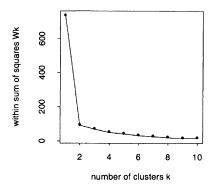
\includegraphics[width=0.4\textwidth]{elbow_clusters.png}
\caption{Demonstration of the elbow clustering selection [ref].}
\label{fig:elbow_cluster}
\end{wrapfigure}

Developed by Robert Thorndike \cite{Thorndike1953} in 1953, this approach looks to plot the inter-cluster sum of squared error verses the number of clusters.  In many clustering applications, the average inter-cluster error will begin to drop significantly and then begin to asymptotically decrease.  The number of clusters is chosen at this "elbow."  \ref{fig:elbow_cluster} demonstrates a this elbow.  In the image, the number of clusters selected is 2.  A common problem with this approach is that the elbow can not always be unambiguously identified.

\bigskip
\noindent
\textbf{Information criterion} \\
An information based approach to selecting the number of clusters is to use either the Akaike information criterion \cite{Akaike1974} or the Bayesian information criterion \cite{Schwarz1978}.  There exist other information criterions, but they do not have the ubiquity of the prior two criterions.  Both the Akaike and the Bayesian criterion seek to determine the number of clusters by imposing a tradeoff between the goodness of fit and the number of model parameters.  For our work, goodness of fit can be measured by the log likelihood of the data to the Gaussian clusters and the number of model parameters is simply the number of models.  

\bigskip
\noindent
\textbf{Cross-validation} \\
TODO WRITE ON CROSS-VALIDATION METHOD


\bigskip
\noindent
\textbf{Silhouette} \\
Silhouette \cite{Rousseuw1987} scores are another method of selecting the number of clusters.  A silhouette score balances the tradeoff between the average dissimilarity between all data points for a given cluster and the average dissimilarity to the data points of the next nearest cluster.  The silhouette score is defined as

\begin{equation}
s(i) = \frac{b(i) - a(i)}{max\{a(i), b(i)\}}.
\end{equation}

$a(i)$ is the average dissimilarity between data point $i$ and all other points within the cluster $i$ is assigned.  $b(i)$ is the average dissimilarity between data point $i$ and all other points within the nearest cluster that does not contain $i$.  The optimal number of clusters is then chosen by finding the maximum silhouette score amongst multiple possible values of K.  Because mixture of Gaussians is a soft cluster assignment algorithm (each point has a likelihood to be assigned to each cluster instead of belonging to one single cluster), we consider the assignment of each point to be only the Gaussian from which it is most likely modeled.

The best method for selecting the optimal number of clusters is an open problem.  Different datasets and different clustering methods may require different criterions to determine the optimal number of clusters.  Since our approach is mostly unsupervised, we do not have the luxury of determining what criterion works best for our data.   

The doctoral thesis \cite{Yan2005} of Yan broached the topic of best clustering criterion and showed significant variation between clustering criterions.  Of these criterions, silhouette based cluster selection was consistently one of the best selection criterions.  Given the variability in selection techniques and combined with Yan's findings, we feel confident that Silhouette scores provide an adequate cluster selection criterion.

\subsection{Sample representative clusters and a discussion about them}

This section visually demonstrates a few of the clusters extracted from our datasets using the time series mixture of Gaussian's approach.  These residual clusters were chosen from each dataset and from different base forecasting approaches.  The images shown here are from a mix of base forecasters without regard to the forecaster's accuracy.  Such clusters have been generated for every combination of dataset and forecaster residuals.

\ref{fig:merl_clusters} is a set of clusters from a residual time series of MERL dataset extracted using the SVM forecaster.  The residuals are from a time series forecasting horizon of 20 minutes (two time steps).  The extracted window length is 70 minutes (seven time steps).  These clusters were taken from the top 10\% of the MERL data residuals.

\begin{figure}
	\begin{center}
		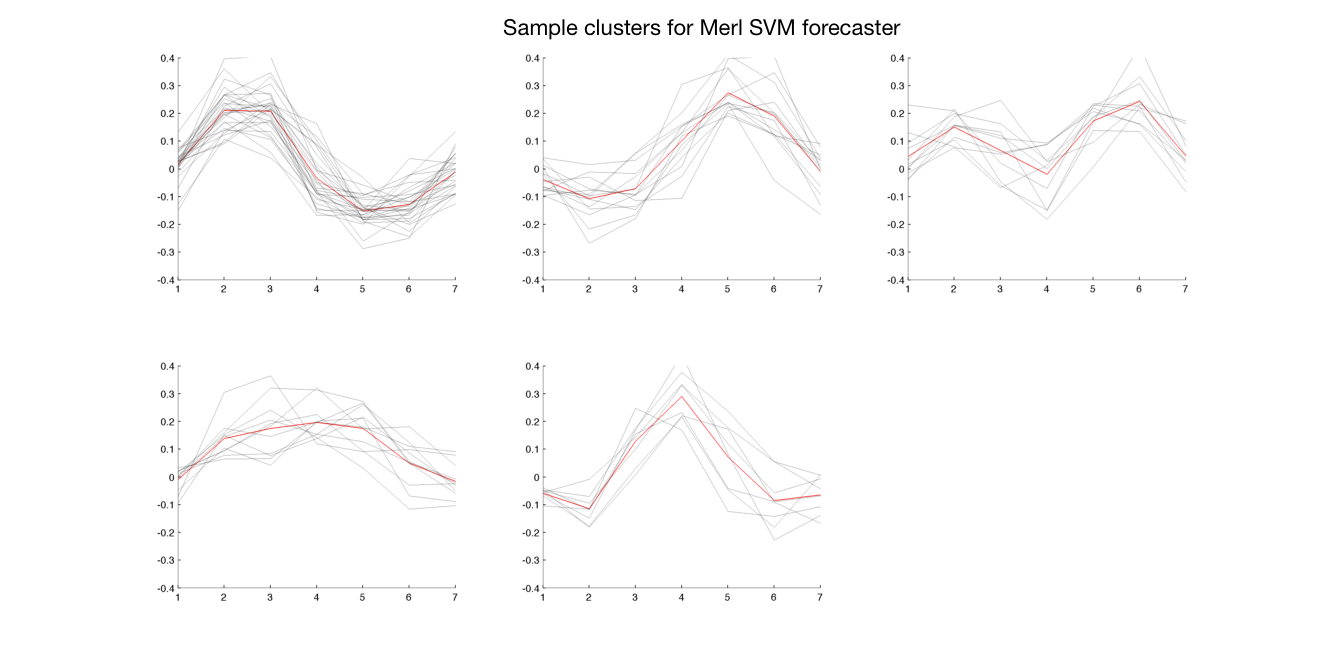
\includegraphics[width=1.00\textwidth]{merl_sample_clusters_svm.png}
	\end{center}
	\caption{Extracted residuals from the MERL dataset.  Data was taken from the top 10\% of the SVM forecaster's residuals.  The red line in the center of the clusters represents the cluster average.}
	\label{fig:merl_clusters}
\end{figure}

\begin{figure}
	\begin{center}
		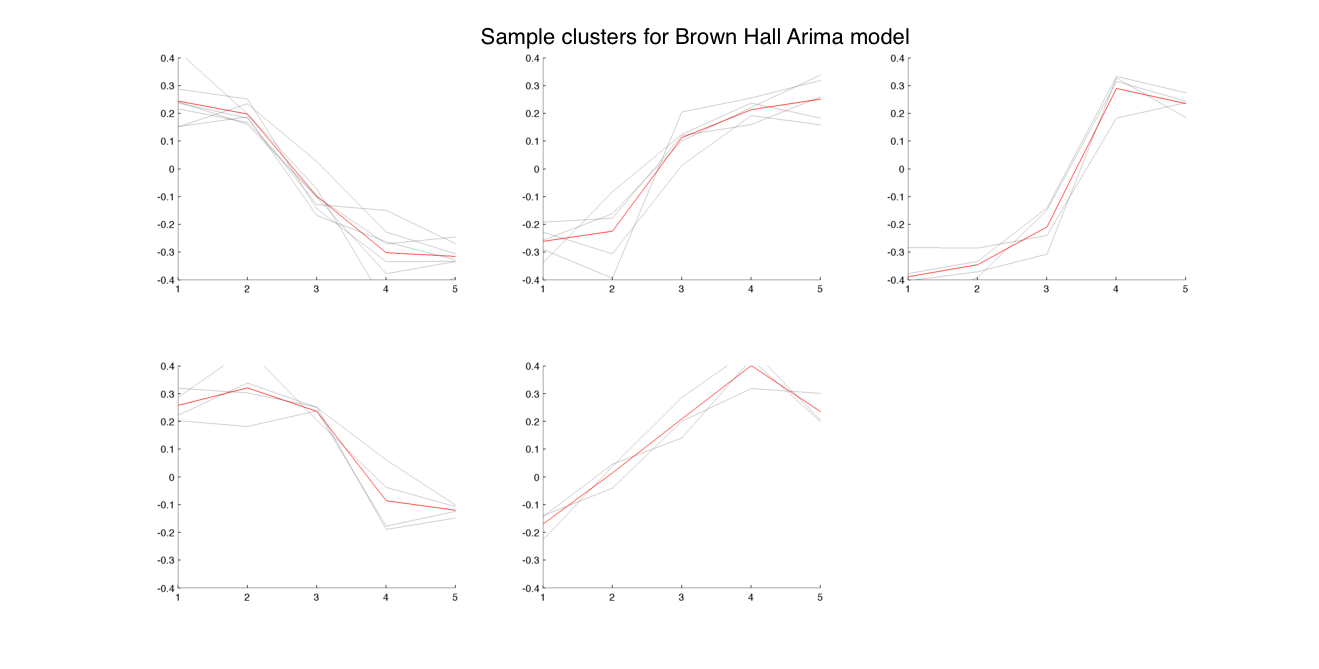
\includegraphics[width = 1.0\textwidth]{brown_sample_clusters_arima.png}
	\end{center}
	\caption{Extracted residuals from the Brown dataset.  Data was taken from the top 10\% of the ARIMA forecaster's residuals.  The red line in the center of the clusters represents the cluster average.}
	\label{fig:brown_clusters}
\end{figure}

\ref{fig:brown_clusters} is the set of clusters from the Brown dataset extracted from the ARIMA forecaster.  The clusters from the dataset were taken from the top 10\% of the Brown data residuals.  Notice how these clusters, unlike the clusters from \ref{fig:merl_clusters} do not begin nor end with a residual value of zero.  This likely means that the true residuals are longer in length than those displayed here.  However, our method of silhouette score maximization returned this set as the best.  Most likely this is due to non-consistent residual behavior if the extracted residual window is increased.
  
\begin{figure}
	\begin{center}
		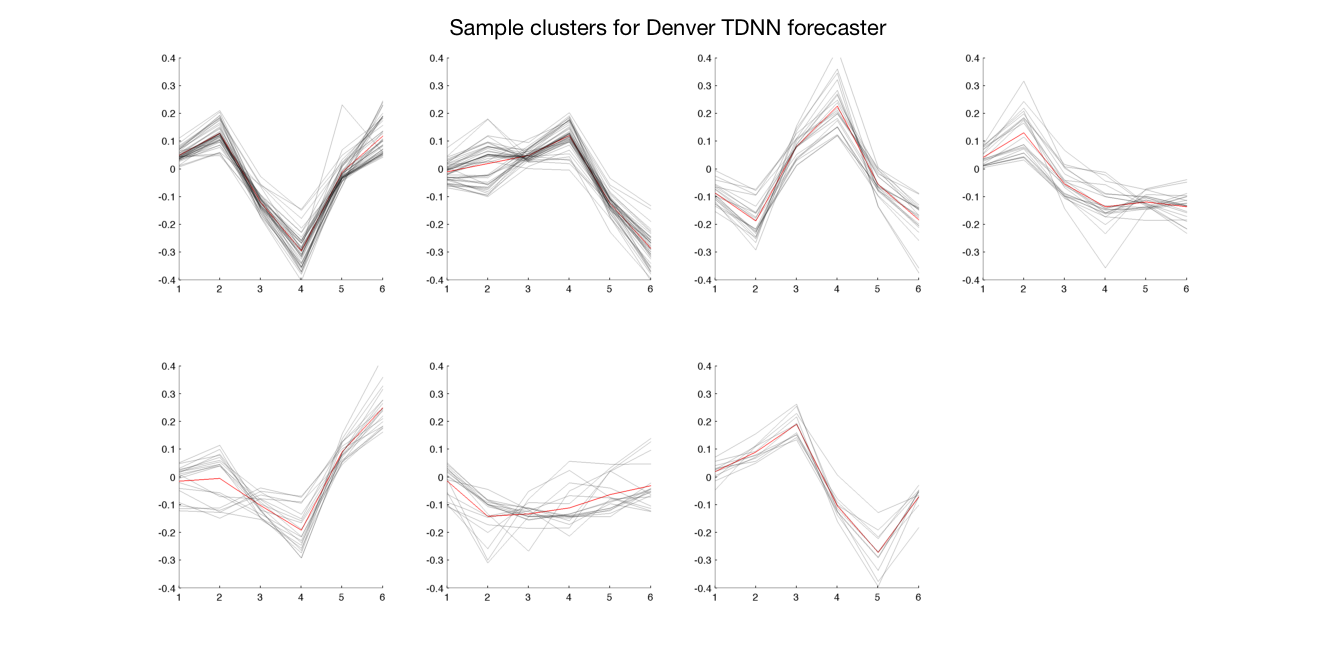
\includegraphics[width=1.0\textwidth]{denver_sample_clusters_tdnn.png}
	\end{center}
	\caption{Extracted residuals from the Denver dataset.  Data was taken from the top 10\% of the TDNN forecaster's residuals.}
	\label{fig:denver_clusters}
\end{figure}

\ref{fig:denver_clusters} displays the set of modeled clusters from the Denver dataset extracted from the TDNN forecaster.  These clusters were taken from the top 10\% of the forecaster's residuals.  The time series within the Denver dataset correspond to 30 minute intervals.  Thus, the clusters shown in \ref{fig:denver_clusters} demonstrate events that occur over at least 3 hours (six time steps).  Also, some of the clusters begin or end with a 0 residual, but others drift higher or lower.  We believe this demonstrates events which may not have finished during the duration of the clusters demonstrated here.  Ideally we would like to have clusters long enough to fit the entire event, but short enough that they don't contain "normal" behavior.  Clusterings such as this demonstrate a scenario where modeling these clusters through a non-fixed length technique may lead to better results.

Also, notice how some of the clusters above show certain member activities which are somewhat dissimilar from the red cluster line.  While we didn't implement it in this work, it is certainly feasible to extract outlier (or dissimilar) activities from the potential pool of activities and rerun the mixture of Gaussians algorithm.  This sort of outlier extraction would likely lead to slightly better anomaly models.

Finally, we believe that the structure demonstrated from these clusters again leads further credibility to the residual data containing some information about the activity or anomaly that generated the data.  These residual clusters do not appear to be simply the product of random noise.  


\subsection{ABCF derived}
\label{sec:abcf}
Here we present the math behind our Anomaly Bayesian combined forecasting algorithm.  Similar to the Bayesian combined forecaster introduced in Chapter 4, our ABCF algorithm is recursive and computationally efficient.  

We present the algorithm using two anomaly event models $a$ and $b$ with a background model $c$.  Extending the algorithm to work for any number of algorithms is apparent from this presentation.  For our work, the models $a$ and $b$ are modeled anomalies from our time series mixture of Gaussians; however this derivation allows the models to be any of a stochastic time series model such that it is possible to compute $p(x_{t} | a^{(i)}_{t})$.  Finally, the model $c$ is assumed to be a background model which allows for the computation of $p(c_{t}|x_{t})$.  

Let $a_{t}^{(i)} = $ the event that model $a$ is active at time $t$ at index $i$ and $b_{t}^{(i)} = $ the event that model $b$ is active at time $t$ at index $i$.  Both anomalies $a$ and $b$ have a known length defined by the function $len(a)$ or $len(b)$.  For each time $t$ we call the data that generated $t$ as event $e$.  Because $a$ and $b$ are the only anomalies modeled, $e$ can be either ${a^{(i)}_{t}}$, ${b^{(i)}_{t}}$ or $c$ for any $i$.

Thus, we know that

\begin{equation}
p(e_{t}) = 1.
\end{equation}

Since, every $e_{t}$ is generated from either $a$, $b$, or $c$, we force (through normalization)

\begin{equation}
\sum_{i}^{len(a)} p(a_{t}^{(i)}|x_{t}, \ldots, x_{1}) + \sum_{i}^{len(b)} p(b_{t}^{(i)}|x_{t}, \ldots, x_{1}) + p(c_{t}|x_{t}, \ldots, x_{1}) = 1.
\label{eq:pabc}
\end{equation}

The goal of this forecaster is then to find each of $p(a_{t + 1}^{(i + 1)})$, $p(b_{t + 1}^{(i + 1)})$, and $p(c_{t + 1}).$  Given these model likelihoods, we can then produce a final forecast in a way similar to BCF in chapter 4 by either using the most likely model or producing an aggregate forecast from each model.

From Bayes rule we have the following equation 

\begin {equation}
p(a_{t + 1}^{(i + 1)}|x_{t + 1}, \ldots, x_{1}) =
		\frac{p(x_{t + 1}|a^{(i + 1)}_{t + 1}, x_{t}, \ldots, x_{1}) p(a_{t + 1}^{(i + 1)}|x_{t}, \ldots, x_{1})}
	       {p(x_{t + 1})}.
\label{eq:update_bayes}
\end{equation}

To find $p(a_{t + 1}^{(i + 1)}|x_{t + 1}, \ldots, x_{1})$ we need to compute $p(x_{t + 1}|a^{(i + 1)}_{t + 1}, x_{t}, \ldots, x_{1})$,  $p(a_{t + 1}^{(i + 1)}|x_{t}, \ldots, x_{1})$ and $p(x_{t + 1})$.

Computing $p(x_{t + 1})$ is straight forward from the law of total probability

\begin{equation}
	\begin{split}
		p(x_{t + 1}) = \sum_{i}^{len(a) - 1}p(x_{t + 1}|a_{t + 1}^{(i + 1)}, x_{t}, \ldots, x_{1})
						   p(a_{t + 1}^{(i + 1)}|x_{t}, \ldots, x_{1}) + \\
				      \sum_{i}^{len(b) - 1}p(x_{t + 1}|b_{t + 1}^{(i + 1)}, x_{t}, \ldots, x_{1}) 
						   p(b_{t + 1}^{(i + 1)}|x_{t}, \ldots, x_{1}) + \\
	        			      p(x_{t + 1}|c_{t + 1}, x_{t}, \ldots, x_{1})p(c_{t + 1}|x_{t}, \ldots, x_{1}).
	\end{split}
\end{equation}

The computation for $p(x_{t + 1}|a^{(i + 1)}_{t + 1}, x_{t}, \ldots, x_{1})$ is performed directly by computing the likelihood of a new data point $x_{t + 1}$ for model $a$ at offset $i + 1$.

Finally, the calculation of $p(a_{t + 1}^{(i + 1)}|x_{t}, \ldots, x_{1})$ is from an earlier forecast and is what gives our algorithm its recursive nature.  We pass the posterior of all values of $a_{t}$ to the priors of $a_{t + 1}.$  Thus $p(a_{t + 1}^{(i + 1)}|x_{t}, \ldots, x_{1})$ is simply a passed value from the last time step in our algorithm.  Specifically we define 

\begin{equation}
	p(a_{t + 1}^{(i + 1)} | x_{t}, \ldots, x_{1}) = 
		\begin{cases}
			p(a_{t}^{(i)}|x_{t}, \ldots, x_{1}) & : i < len(a) \\
			0 & : otherwise.
		\end{cases}
	%\right
\end{equation}

In the present of an event we pass along the likelihood of that even to the next time step and recompute the posterior of that event.  The prior for the start of each event is a user tunable parameter.  

\begin{equation}
	\begin{split}
		p(a_{t + 1}^{(1)}|x_{t}, \ldots, x_{1}) = p(a_{t + 1}^{(1)}) = \theta_a \\
		p(b_{t + 1}^{(1)}|x_{t}, \ldots, x_{1}) = p(b_{t + 1}^{(1)}) = \theta_b
	\end{split}
\end{equation}

\noindent
Equation \ref{eq:update_bayes} now turns into 

\begin{equation}
p(a_{t + 1}^{(i + 1)}|x_{t + 1}, \ldots, x_{1}) =
		\frac{p(x_{t + 1}|a^{(i + 1)}_{t + 1}, x_{t}, \ldots, x_{1}) p(a_{t + 1}^{(i)}|x_{t}, \ldots, x_{1})}
	       {p(x_{t + 1})}.
\label{eq:update_prior}
\end{equation}

\noindent
The prior is now $p(a_{t + 1}^{(i)}|x_{t}, \ldots, x_{1})$ which does not depend on $x_{t + 1}$ or $a^{i + 1}$.  Performing equation \ref{eq:update_prior} on both $a$ and $b$ and computing $c$ directly yields equation \ref{eq:pabc} which, when normalized equals $1$.  The normalized values of $p(a_{t + 1}^{(i + 1)}$, $p(b_{t + 1}^{i + 1})$, and $p(c)$ are then used to produce either a most likely or weighted aggregate forecast.

%%%%%%%%%%%%%%%%%%%%%%%%%%%%%%%%%%%%%%%%%%%%%%%%%
%Demonstration of ABCF
%%%%%%%%%%%%%%%%%%%%%%%%%%%%%%%%%%%%%%%%%%%%%%%%%

\begin{figure}[!t]
	\begin{center}
		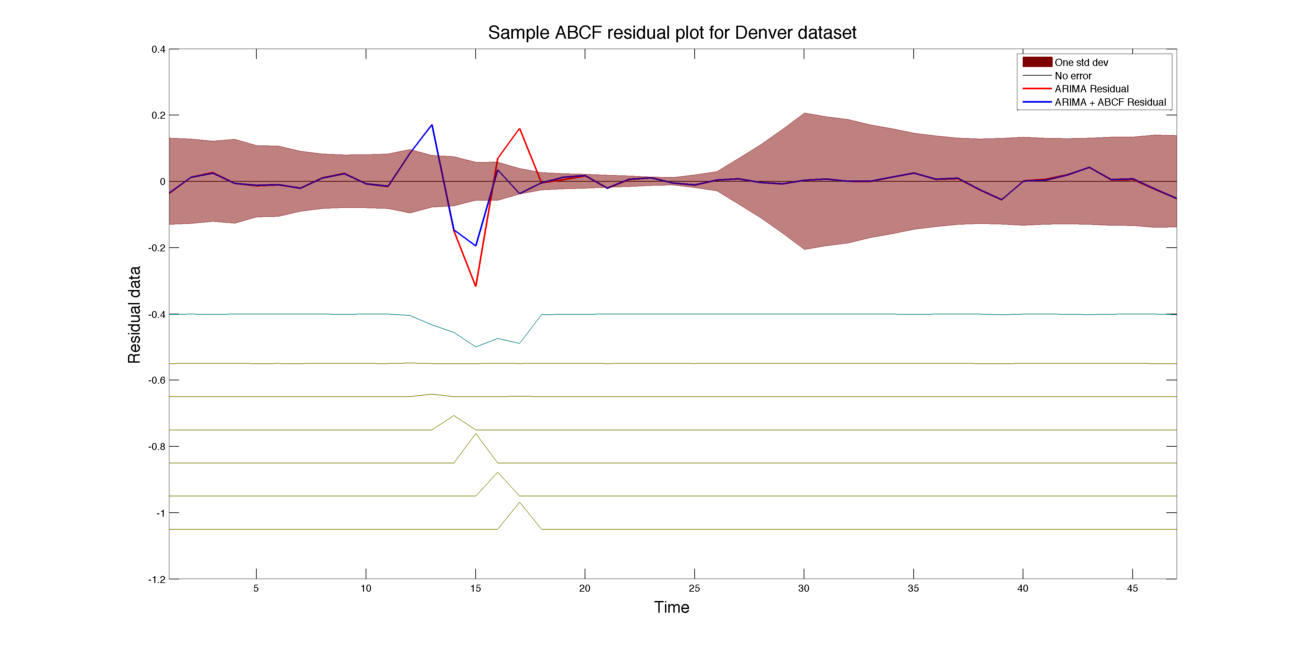
\includegraphics[width=1.0\textwidth]{sample_residual_plot_dataset_Denver.png}
	\end{center}
	\caption{Sample residual and the respective probabilities of each time step for the base forecaster and the a single activity model.  The teal line represents the likelihood of the background ARIMA model.  The tan lines correspond to the likelihood each time step from one of the anomaly clusters.}
	\label{fig:sample_abcf_residual}
\end{figure}

\subsection{Demonstration of ABCF}
\ref{fig:sample_abcf_residual} is a demonstration of ABCF.  This figure displays a sample time frame (in blue) from the Denver dataset along with the corresponding region for one standard deviation of noise from a best fit ARIMA forecaster with a horizon of two time steps.  The teal line below the graph is the likelihood of the background ARIMA model accurately representing the residual data from the set of clustered anomalies.  The remaining tan lines are the individual likelihoods of each time step of a given clustered anomaly shown in \ref{fig:sample_cluster}  

The red line is the resulting ABCF forecast to the residual.  Ideally the residual should be completely zero, thus resulting in no forecasting error.  At approximately time 10, an anomalous event begins to occur.  The ABCF algorithm takes a few time steps to identify this anomaly and determine that the background ARIMA forecaster is no longer accurate.  We see this effect by noticing the teal line's reduction in likelihood from approximately time step 12 to time step 17.  During this time all other extracted clusters are attempting to fit the anomaly.

\begin{wrapfigure}{R}{0.3\textwidth}
\centering
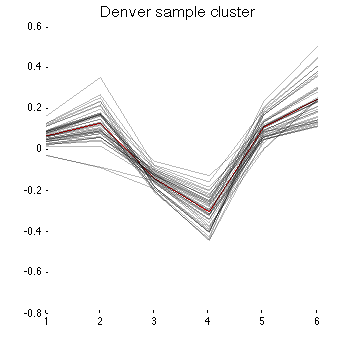
\includegraphics[width=0.25\textwidth]{denver_sample_cluster.png}
\caption{Extracted sample clustered anomaly.}
\label{fig:sample_cluster}
\end{wrapfigure}

The recursive nature of our likelihood time step propagation in the ABCF algorithm is apparent in the tan lines of this sample figure.  At time step 13, there is a slight perturbation in the second tan line.  This perturbation continues to rise both in value (indicating an increase in likelihood that this cluster is active) and time along the anomaly.  Finally at about time step 18, the model is finished.  At this point the likelihood of the background model begins to rise again and eventually the background model (the teal line) is once again the most prevalent model amongst all the extracted anomalies.

\ref{fig:sample_abcf_residual} displays a significant improvement in RMSE-ONAN.  While the early stages of the anomaly show no improvement, the residual error during the middle of the anomaly is roughly halved and the residual error at the end of the anomaly is nearly zero.  \ref{fig:sample_abcf_denver} shows the final result of this forecast window.  The ARIMA forecaster is delayed in its forecast response to the anomaly, but because such an anomaly was commonly seen within this dataset, the ABCF algorithm is able to estimate the anomaly and improve forecasting accuracy during the remainder of the anomaly.

\begin{figure}[!h]
	\begin{center}
		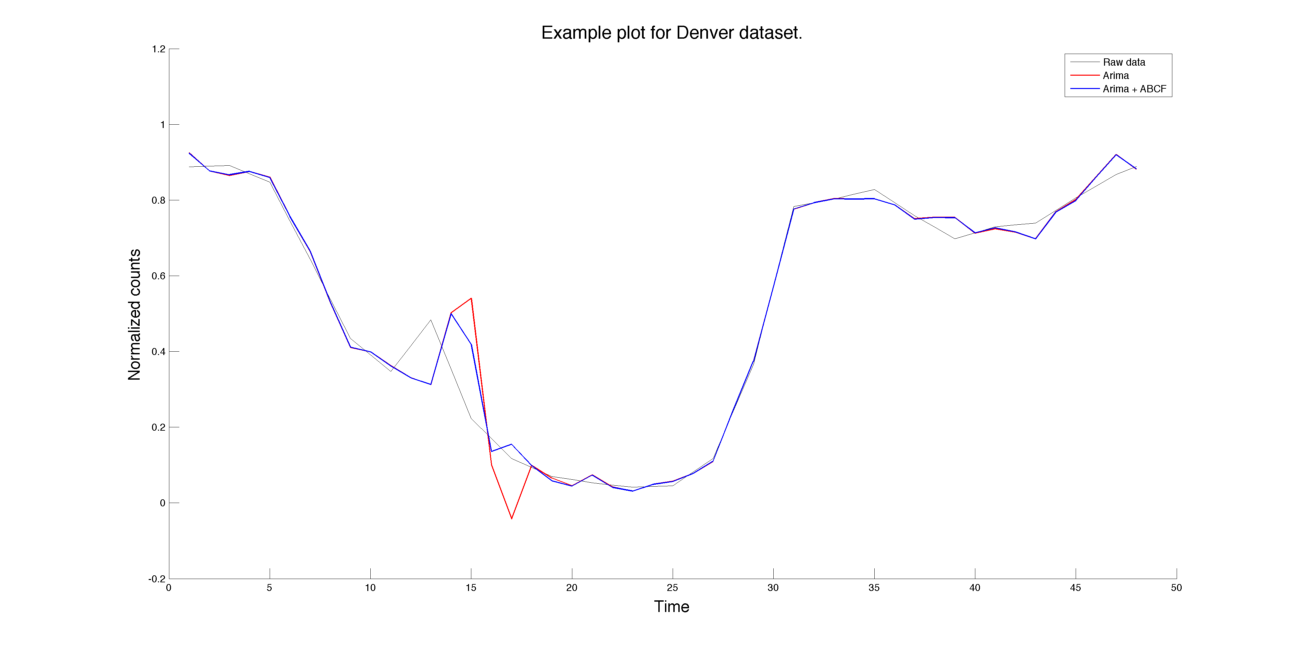
\includegraphics[width=1.0\textwidth]{sample_plot_Denver.png}
	\end{center}
	\caption{Two horizon time step results when applying ABCF to an ARIMA forecaster for a segment of the Denver dataset.}
	\label{fig:sample_abcf_denver}
\end{figure}


%%%%%%%%%%%%%%%%%%%%%%%%%%%%%%%%%%%%%%%%%%%%%%%%%
%Results of ABCF
%%%%%%%%%%%%%%%%%%%%%%%%%%%%%%%%%%%%%%%%%%%%%%%%%
\subsection{Results of ABCF}
Because the results are given over multiple forecasting horizons with several base forecasters and multiple forecasting metrics, we believe that tables are not an adequate format to display our results.  Also, since the number of potential images to display about the improvements due to ABCF is quite large, we provide a few images here to demonstrate our results and put the remaining images in Appendix \ref{app:results} for the interested reader.  The images presented here first demonstrate our ABCF technique applied to the Denver dataset.  Later images in this section display more aggregated results for each of the datasets, forecasting models and forecasting metrics.

\bigskip
\noindent \textbf{Denver dataset results} 

\begin{figure}[!b]
	\begin{center}
		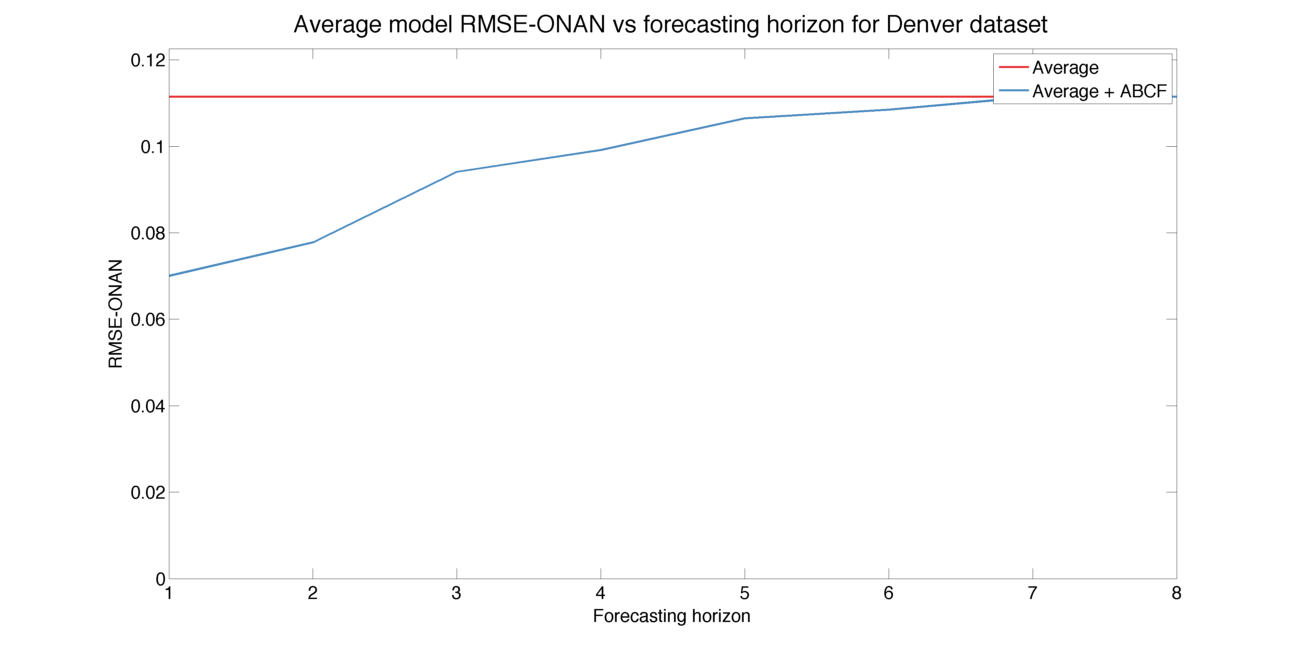
\includegraphics[width=1.0\textwidth]{rmseonan_average_abcf_Denver.png}
	\end{center}
	\caption{RMSE-ONAN vs forecasting horizon for Average model and Average + ABCF on the Denver dataset}
	\label{fig:average_abcf_rmseonan_denver}
\end{figure}

\ref{fig:average_abcf_rmseonan_denver} demonstrates the improvements to the RMSE-ONAN metric of applying our ABCF algorithm to the average forecasting algorithm for the Denver dataset.  We found our largest improvements came with the historic average model.  The reason likely being that any activities or consistent deviations from normal behavior show up in the average model.  These behaviors are well represented in the residuals and thus make good candidate models for our ABCF model.

\begin{figure}[!h]
	\begin{center}
		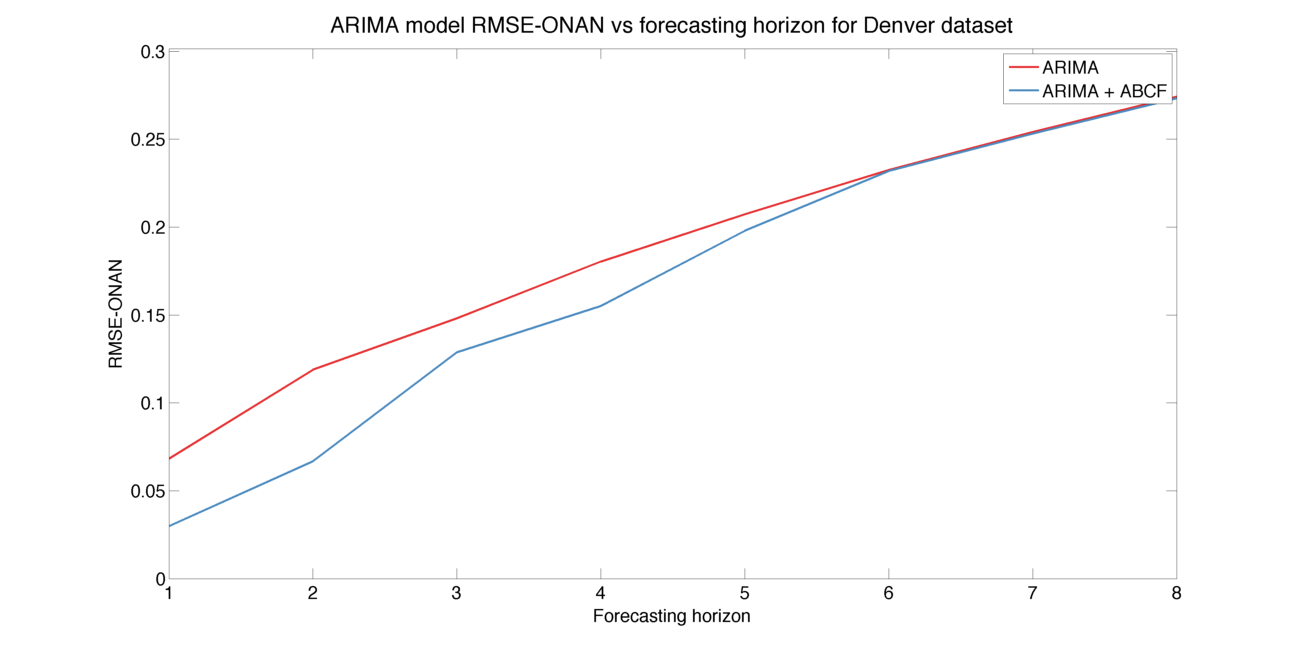
\includegraphics[width=1.0\textwidth]{rmseonan_arima_abcf_Denver.png}
	\end{center}
	\caption{RMSE-ONAN vs forecasting horizon for ARIMA model and ARIMA + ABCF on the Denver dataset}
	\label{fig:arima_abcf_rmseonan_denver}
\end{figure}

\begin{figure}[!h]
	\begin{center}
		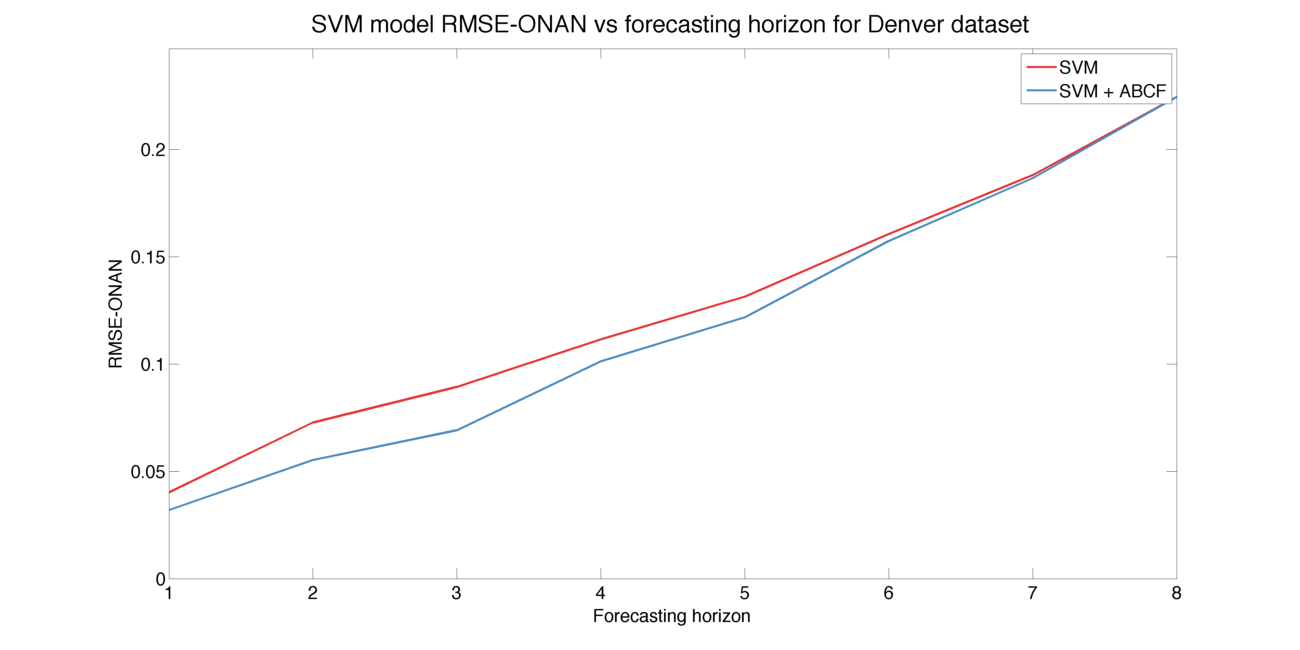
\includegraphics[width=1.0\textwidth]{rmseonan_svm_abcf_Denver.png}
	\end{center}
	\caption{RMSE-ONAN vs forecasting horizon for SVM model and SVM + ABCF on the Denver dataset}
	\label{fig:svm_abcf_rmseonan_denver}
\end{figure}

\begin{figure}[!h]
	\begin{center}
		\includegraphics[width=1.0\textwidth]{rmseonan_TDNN_abcf_Denver.png}
	\end{center}
	\caption{RMSE-ONAN vs forecasting horizon for TDNN model and TDNN + ABCF on the Denver dataset}
	\label{fig:tdnn_abcf_rmseonan_denver}
\end{figure}

\ref{fig:arima_abcf_rmseonan_denver}, \ref{fig:svm_abcf_rmseonan_denver}, and \ref{fig:tdnn_abcf_rmseonan_denver} display the improvement to the RMSE-ONAN metric when applying ABCF to an ARIMA, SVM and TDNN forecaster on the Denver dataset.  While smaller, the improvements are still significant and present out to roughly six time steps.  Interestingly, the TDNN model showed much more mixed results.  Generally applying ABCF resulted in better results, but this was not always the case.  We believe this is due to the significantly more volatile forecasting results of the TDNN model.  From \ref{fig:rmseplotdenver} we know that the TDNN model was generally the worst forecaster for the Denver dataset with substantial variance in forecasting.  Also, Neural Networks are known to suffer a lack of robustness to outliers \cite{connor1994}.  Techniques have been developed to increase outlier robustness, but we did not explore them for this work.

\begin{figure}[!h]
	\begin{center}
		\includegraphics[width=1.0\textwidth]{rmseonan_abcf_bcf_Denver.png}
	\end{center}
	\caption{RMSE-ONAN vs forecasting horizon for BCF-TS model and BCF-TS + ABCF on the Denver dataset}
	\label{fig:bcf_abcf_rmseonan_denver}
\end{figure}

\begin{figure}[!h]
	\begin{center}
		\includegraphics[width=1.0\textwidth]{rmseonan_improvement_for_each_forecaster_for_Denver.png}
	\end{center}
	\caption{}
	\label{fig:rmseonan_improve_denver}
\end{figure}

\ref{fig:bcf_abcf_rmseonan_denver} shows the results of applying ABCF to the BCF-TS model introduced in the previous chapter.  In this ensemble forecaster, the ABCF technique is still able to find enough structured anomalies to reduce the RMSE-ONAN metric.  Despite BCF-TS being an ensemble with TDNN included, the sensitivity to outliers has been reduced and ABCF demonstrates an improvement up to 6 forecasts into the future.  Forecasts 7 or 8 time steps appear to be slightly worse applying ABCF.  This is not a surprising result as the extracted activities for the Denver dataset were 6 time steps in length.

An aggregate of the prior graphs as a percentage of improvement if shown in \ref{fig:rmseonan_improve_denver}.  In almost all cases, applying ABCF to a base forecaster for the Denver dataset resulted in forecasting improvement to RMSE-ONAN.  The improvements generated from ABCF are highest on short forecasts and drop to roughly zero for forecasts longer than 6 time steps into the future.  For every forecaster we achieve an improvement of at least 20\% at one time step horizon.  This improvement is still 15-20\% for most forecasters at three time steps.  Put in context, the forecasting accuracy of many anomalous traffic events has improved 15 - 20\% over 3 hours into the future.


%%%%%%%%%%%%%%%%%%%%%%%%%%%%%%%%%%%%%%%%%%%%%%%%%
%Aggregated Results
%%%%%%%%%%%%%%%%%%%%%%%%%%%%%%%%%%%%%%%%%%%%%%%%%
\bigskip
\noindent \textbf{Remaining aggregated results} 

\begin{figure}[!h]
	\begin{center}
		\includegraphics[width=1.0\textwidth]{rmseonan_improvement_for_each_forecaster_for_Merl.png}
	\end{center}
	\caption{}
	\label{fig:rmseonan_improve_merl}
\end{figure}

\begin{figure}[!h]
	\begin{center}
		\includegraphics[width=1.0\textwidth]{rmseonan_improvement_for_each_forecaster_for_Brown.png}
	\end{center}
	\caption{}
	\label{fig:rmseonan_improve_brown}
\end{figure}


\ref{fig:rmseonan_improve_merl}, and \ref{fig:rmseonan_improve_brown} show the percentage improvement to the RMSE-ONAN metric using ABCF to supplement a given base forecaster.  The improvement due to ABCF varies greatly based on both forecaster and dataset.  As expected, ABCF improves a historic average forecaster by the largest margin.  The improvement is over 70\% on the Denver dataset and still over 25\% on the Brown hall set.

At the one and two time step forecasting horizon, both BCF and our IBCF algorithm introduced in the last chapter are amongst the forecasters that benefit the least from applying ABCF.  We believe the smaller improvement margins are due the properties of ensemble forecasters.  Such forecasters will change forecasting models based on the structure of the dataset at any given time.  These changes may not lead to clusters which are clean and thus as easily able to be modeled.  I

As ABCF is an ensemble forecaster, it can make no guarantees on its improvement.  For forecasts one time step ahead using the SQEONAN metric on the Brown Hall dataset, the BCF forecaster out performed a hybrid BCF + ABCF forecast.  From our results, we found that such negative effects on forecasting performance were rare, occurring in only a few of our examples.

\ref{fig:rmse_improve_merl}, \ref{fig:rmse_improve_brown}, and \ref{fig:rmse_improve_denver} show the improvement of applying ABCF to each model using RMSE. \ref{fig:mase_improve_merl}, \ref{fig:mase_improve_brown}, and \ref{fig:mase_improve_denver} show the improvements of ABCF using MASE.  These images demonstrate that our forecasting improvements when applying ABCF are typically quite small (<5\%) when considering the entire time series.  These improvements are tied to the density of anomalies within the dataset.  A dataset with more anomalies relative to the forecaster will experience a larger overall improvement in forecasting error.

Overall these results demonstrate that ABCF has the power to improve anomaly forecasting while having a little to no detrimental effect on the overall forecasting performance of our forecaster.  Our worse case scenario occurred when applying ABCF to an SVM forecaster on the MERL dataset and for a forecasting horizon of 2 and 3 we experienced 3 - 4\% error in forecasting performance.  However, in almost all other scenarios ABCF improved the overall forecasting accuracy and greatly improved the accuracy of anomaly forecasting as measured by our SQEONAN metric.

  
\begin{figure}[!h]
	\begin{center}
		\includegraphics[width=1.0\textwidth]{rmse_improvement_for_each_forecaster_for_Merl.png}
	\end{center}
	\caption{}
	\label{fig:rmse_improve_merl}
\end{figure}

\begin{figure}[!h]
	\begin{center}
		\includegraphics[width=1.0\textwidth]{rmse_improvement_for_each_forecaster_for_Brown.png}
	\end{center}
	\caption{}
	\label{fig:rmse_improve_brown}
\end{figure}

\begin{figure}[!h]
	\begin{center}
		\includegraphics[width=1.0\textwidth]{rmse_improvement_for_each_forecaster_for_Denver.png}
	\end{center}
	\caption{}
	\label{fig:rmse_improve_denver}
\end{figure}

\begin{figure}[!h]
	\begin{center}
		\includegraphics[width=1.0\textwidth]{mase_improvement_for_each_forecaster_for_Merl.png}
	\end{center}
	\caption{}
	\label{fig:mase_improve_merl}
\end{figure}

\begin{figure}[!h]
	\begin{center}
		\includegraphics[width=1.0\textwidth]{mase_improvement_for_each_forecaster_for_Brown.png}
	\end{center}
	\caption{}
	\label{fig:mase_improve_brown}
\end{figure}

\begin{figure}[!h]
	\begin{center}
		\includegraphics[width=1.0\textwidth]{mase_improvement_for_each_forecaster_for_Denver.png}
	\end{center}
	\caption{}
	\label{fig:mase_improve_denver}
\end{figure}

\newpage


%%%%%%%%%%%%%%%%%%%%%%%%%%%%%%%%%%%%%%%%%%%%%%%%%
%Future work
%%%%%%%%%%%%%%%%%%%%%%%%%%%%%%%%%%%%%%%%%%%%%%%%%
\subsection{Future unexplored work on ABCF}
While we are happy with the current status of the ABCF algorithm, we would recommend the following potential avenues for improvement.

\begin{enumerate}
	\item Explore different data extraction and clustering techniques.  More research into techniques which do not rely on fixed length extracted residual windows.  If a reliance on a sliding window extraction method is to continue, then trimming or growing the sliding window based on the shape of any potential residual.  Another possibility would be to use a sparse dictionary encoding technique to determine the a best dictionary of anomalies for each residual time series.
	
	\item Acquire and test with other datasets.  The datasets presented here give a baseline to test from, but we realize that it does not represent all types of human traffic data.  We would like to test from a traffic dataset with shorter time scales (recall that the Denver dataset is every 30 minutes).  Also we would like to have other types of building data.  Do our approaches work with apartments or government buildings?  Rich building datasets would allow us to answer this question and may lead to improvements in our approach based on the results.
	
	\item Test with additional forecasters.  The four base forecasters we've selected represent a good base, but other forecasters, such as wavelet based or Markov based, may produce some unintuitive results.  We are especially interested in a forecaster or cluster which has a non-Gaussian noise distribution.  Our algorithm allows for any noise distribution, but all of our tests have only been with Gaussian noise.
\end{enumerate}



\chapter{conclusion}

The utility of time series forecasting is likely to continue to grow.  Fully automated heating and cooling systems utilizing multiple power sources are becoming more prevalent.  Autonomous vehicles may soon become ubiquitous instead of simply a science fiction fantasy.  Traffic light control centers are becoming centralized allowing for total control of a large system.  However, despite the growing need for time series forecasting of traffic systems, we found little literature on repeating anomalies or activities.  This dissertation focused on two essential areas of time series clustering: improved ensemble forecasts and improved detection and forecasting during the presence of anomalies.  

\bigskip
\noindent \textbf{Improved ensemble forecasts}\\
In \ref{ch:BCF} we gave an in-depth discussion of Bayesian Combined Forecasting and showed the results of that ensemble forecasting model when applied to three different traffic datasets (two building datasets and one vehicle dataset).  We demonstrated for most forecasting horizons and for each of our datasets that BCF is a good general purpose forecaster.  It obtained a forecasting accuracy that was nearly as good or better than the best component forecaster (SVM, ARIMA, TDNN, Average).  

We then demonstrated a few modifications to BCF which were primarily targeted at improving the accuracy of forecasting horizons $ > 1$.  These changes involved computing a different model error distribution based on the forecasting horizon along with a model selection thresholding technique.  These implemented changed improved the accuracy of the BCF algorithm by approximately 5 - 10\% for both Brown and MERL datasets with the Denver dataset showing much higher improvements.  

 \bigskip
\noindent \textbf{Anomaly forecasting}\\
In this work we looked to solve the problem of forecasting during the presence of anomalies or repeated non-periodic activities.  Examples of such activities are sporting events for vehicle traffic data.  Sporadic meetings or canceled classes are examples for building data.  Traditional techniques either ignore such events or use dynamic models that are typically unable to accurately respond to such events.  

This work built on the inaccuracies of other models during such activities to first detect and model these activities.  We described a simple activity extraction method using residual data.  We then modeled these activities using a time-series mixture of Gaussians.  These time-series Gaussian clusters were then incorporated into a new recursive ensemble model.  Because, by their very nature, these activities are uncommon in the data we saw little improvement in traditional forecasting metrics such as RMSE and MASE.  For this reason, to better represent these activities we introduced a new time-series forecasting metric RMSE-ONAN.  This metric measures the effects of these activities.  

Using RMSE-ONAN we demonstrated significant forecasting improvements with our ABCF technique.  On some datasets and for some forecasting models the effects were over 50\%.  In almost all forecasting horizons on any model and dataset the results were better or stayed about the same using traditional forecasting metrics.  In our worse case we experienced about a 2\% decrease in overall accuracy.  From these results, we conclude that at least for these datasets there is little reason not to use our anomaly forecasting technique after training a forecasting model.  The accuracy during activities will likely increase significantly with a potential slight improvement in overall accuracy.

%\backmatter

% Use "Advanced" Bibliography Techniques
\bibliography{Final_Thesis}

\appendix{Other results}\label{app:results}
All remaining image results are in this section.  All references are given later in ~\ref{app:references}

\begin{figure}
	\begin{center}
		\includegraphics[width = 1.0\textwidth]{sqeonan_improvement_for_each_forecaster_for_Merl.png}
	\end{center}
	\caption{Percent improvement of applying ABCF to each forecaster for each forecasting horizon for the MERL Hall dataset}
	\label{fig:merl_sqeonan_improvement}
\end{figure}

\begin{figure}
	\begin{center}
		\includegraphics[width = 1.0\textwidth]{sqeonan_improvement_for_each_forecaster_for_Brown.png}
	\end{center}
	\caption{Percent improvement of applying ABCF to each forecaster for each forecasting horizon for the Brown Hall dataset}
	\label{fig:brown_sqeonan_improvement}
\end{figure}

\begin{figure}
	\begin{center}
		\includegraphics[width = 1.0\textwidth]{sqeonan_improvement_for_each_forecaster_for_Denver.png}
	\end{center}
	\caption{Percent improvement of applying ABCF to each forecaster for each forecasting horizon for the Denver dataset}
	\label{fig:denver_sqeonan_improvement}
\end{figure}

\begin{figure}
	\begin{center}
		\includegraphics[width = 1.0\textwidth]{sqeonan_improvement_for_each_dataset.png}
	\end{center}
	\caption{Average percent improvement of applying ABCF to each forecaster to a given dataset.}
	\label{fig:sqeonan_improvement_all_dataset}
\end{figure}

%TODO include RMSE and Mase images


%Reference appendix
\appendix{Figure references}\label{app:references}

%All the figure references are here.
\ref{fig:merl_sqeonan_improvement},
\ref{fig:brown_sqeonan_improvement},
\ref{fig:denver_sqeonan_improvement},
\ref{fig:sqeonan_improvement_all_dataset}

\end{document}
